\documentclass[article,12pt]{elsarticle}
\usepackage[spanish]{babel}
\usepackage[utf8]{inputenc}
\usepackage{amssymb}
\usepackage{flushend}
\usepackage{float}
\usepackage{anysize}
\usepackage{amsmath}
\usepackage{amsfonts}
\usepackage{dcolumn}
\usepackage{amsthm}
\usepackage{caption}
\usepackage{float}
\usepackage{subfigure}
\usepackage{graphicx}
\usepackage{lmodern}
\usepackage{booktabs}
\usepackage{color}
\usepackage{longtable}
\usepackage{rotating}
\usepackage{etoolbox}
\usepackage{comment}
\usepackage{pdflscape}
\usepackage{booktabs}


\date{20 de Noviembre de 2024}
\begin{document}

\begin{frontmatter}
    \title{Laboratorio de Electromagnetismo \\  Proyecto  Final\\ 
        Análisis (electro)magnetohidrodinámico de un fluido reoscópico bajo disposición multimodal de imanes de neodimio }
    \author{Iván Bautista Alvarado$^1$ y Andrés López González$^1$} %Aquí va el nombre de los integrantes que participaron en el informe.
    \address{$^1$ Facultad de Ciencias, Universidad Nacional Autónoma de México, M\'exico CDMX.}


    \begin{abstract}
     Our present study explores the complex interactions within an (electro)magnetohydrodynamic system using an experimental setup consisting of a high-voltage source connected to a pair of copper electrodes submerged in a custom-formulated rheoscopic fluid. This fluid comprises an 8.6\% sodium bicarbonate ($NaHCO_3$) solution, 400 ml of water, and 5 g of pearlescent mica. This configuration generates a conductive fluid, to which currents of 150, 300, and 450 mA were applied, inducing potential differences to observe the effects on the fluid under the influence of an N35-grade neodymium magnet arranged in various polarity and geometric configurations. 

The tests included experiments with a single magnet oriented with either the north or south pole facing upward, pairs of magnets separated by 7 cm with either opposite or identical poles, and configurations of four magnets arranged in a chessboard pattern or with aligned poles. These setups exhibit distinct and highly specific behavioral characteristics depending on the arrangement. Additionally, droplets of a non-conductive tinted liquid were introduced to visualize the flow patterns. 

The results provide an in-depth analysis of how variations in polarity, the number of magnets, and their arrangement affect the behavior of the conductive fluid under differing magnetic and current conditions. This study contributes to a more advanced understanding of complex magnetohydrodynamic systems while highlighting the captivating kalliroscopic patterns produced by the interactions between fields.
    \end{abstract}

    \begin{keyword}
     Electromagnetism; Hydrodinamics; Magnetohydrodinamics; Electrodynamics; Lorentz force; Maxwell ecuations; Navier-Stokes ecuations; Rheoscopic fluid.
    \end{keyword}
\end{frontmatter}

\section*{Resumen}
Nuestro presente estudio explora las complejas interacciones en un sistema (electro)magnetohidrodinámico utilizando una disposición experimental de una fuente de alto voltaje conectada a un par de electrodos de cobre sumergidos en un fluido reoscópico de formulación propia que consiste en una disolución de bicarbonato de sodio ($NaHCO_3$) al 8.6\%, con 400 ml de agua y 5 g de mica perlante. Este conjunto permite la generación de un fluido conductor al cual se aplicaron corrientes de 150, 300 y 450 mA, induciendo diferencias de potencial para observar los efectos en el fluido bajo la influencia de un imán de neodimio de grado N35 en varias configuraciones de polaridad y disposición geométrica. Las pruebas incluyen experimentos con un solo imán con el polo norte o sur orientado hacia arriba, pares de imanes separados a 7 cm con polos opuestos o iguales, y configuraciones de cuatro imanes en arreglo tipo ajedrez y polo igual, que de acuerdo al arreglo presentan características muy particulares en su comportamiento. Además, se añadieron gotas de un líquido tintado no conductor para visualizar los patrones de flujo. Los resultados ofrecen un análisis profundo de cómo las variaciones en la polaridad, número y disposición de los imanes afectan el comportamiento del fluido conductor bajo diferentes condiciones magnéticas y de corriente, contribuyendo a una comprensión más avanzada de los sistemas magnetohidrodinámicos complejos y disfrutando del kalliroscopio que las interacciones entre campos produce.\\

\textit{Palabras clave:} Electromagnetismo; Hidrodinámica; Magnetohidrodinámica; Electrodinámica; Fuerza de Lorentz; Ecuaciones de Maxwell; Ecuaciones de Navier-Stokes; Fluido reoscópico. \\
\hline

\section{Introducción}
    La \textbf{magnetohidrodinámica} (MHD) es una rama de la física que estudia el comportamiento de los fluidos conductores de electricidad, como el plasma, bajo la influencia de campos magnéticos. Está basado en la combinación de los principios de la \textbf{hidrodinámica}, que describe el movimiento de los fluidos y el \textbf{electromagnetismo}, que se ocupa de los efectos de los campos magnéticos sobre las cargas eléctricas y las corrientes.
    
    En la MHD, se asume que el fluido es eléctricamente conductor, lo que significa que puede generar corrientes eléctricas cuando se mueve a través de un campo magnético. Estas corrientes, a su vez, generan fuerzas magnéticas que afectan el movimiento del fluido.
    
    La dinámica de fluídos está descrita por:

    \begin{table}[h!]
\centering
\begin{tabular}{|c|c|}
\hline
\textbf{Ecuación}          & \textbf{Forma Matemática}                                                                                                                                                     \\ \hline
Ecuación de Continuidad    & $\frac{\partial \rho}{\partial t} + \nabla \cdot (\rho \mathbf{v}) = 0$                                                                                                       \\ \hline
Ecuación de Momentum       & $\rho \frac{\partial \mathbf{v}}{\partial t} + \rho (\mathbf{v} \cdot \nabla) \mathbf{v} = -\nabla p + \nabla \cdot \mathbf{\tau} + \rho \mathbf{g} + \mathbf{J} \times \mathbf{B}$ \\ \hline
Ecuación de Inducción      & $\frac{\partial \mathbf{B}}{\partial t} = \nabla \times (\mathbf{v} \times \mathbf{B}) + \eta \nabla^2 \mathbf{B}$                                                                 \\ \hline
Ecuación de Bernoulli      & $\frac{1}{2} \rho |\mathbf{v}|^2 + \rho g h + p + \frac{\mathbf{B}^2}{2\mu_0} = \text{constante}$                                                                             \\ \hline
Ley de Ohm Generalizada    & $\mathbf{J} = \sigma (\mathbf{E} + \mathbf{v} \times \mathbf{B})$                                                                                                            \\ \hline
Ecuación de Navier-Stokes  & $\rho \frac{\partial \mathbf{v}}{\partial t} + \rho (\mathbf{v} \cdot \nabla) \mathbf{v} = -\nabla p + \eta \nabla^2 \mathbf{v} + \rho \mathbf{g} + \mathbf{J} \times \mathbf{B}$ \\ \hline
\end{tabular}
\caption{Ecuaciones fundamentales de la dinámica de fluidos.}
\label{tab:MHD_Ecuaciones}
\end{table}
    
    Centrémonos en el primer término de Navier-Stokes $\rho \left( \frac{\partial \mathbf{v}}{\partial t} + \mathbf{v} \cdot \nabla \mathbf{v} \right)$ representa la aceleración del fluido, considerando tanto el cambio temporal de la velocidad como los efectos no lineales debidos al movimiento del fluido. El segundo término $-\nabla p$ es el gradiente de presión, que describe cómo la presión del fluido actúa para mover el fluido. El tercer término $\eta \nabla^2 \mathbf{v}$: es el término viscoso, que representa la difusión de la velocidad debido a la viscosidad del fluido, es decir, la fricción interna entre las capas de fluido. El cuarto término $\mathbf{f} =\rho \mathbf{g} + \mathbf{J} \times \mathbf{B}$: f representa las fuerzas externas, como la fuerza de Lorentz, la gravedad o cualquier otra fuerza externa aplicada al fluido, en nuestra tabla hemos sustituído directamente la expresión de f de la ecuación original de Navier-Stokes (la cual es $\rho \frac{\partial \mathbf{v}}{\partial t} + \rho (\mathbf{v} \cdot \nabla) \mathbf{v} = -\nabla p + \eta \nabla^2 \mathbf{v} + \textbf{f})$, sin embargo en breve demostraremos por qué es así.
    
    En la MHD se asume que la viscosidad del fluído es nula. así que tenemos la ecuación:
    \begin{equation}
    \rho \left( \frac{\partial \mathbf{v}}{\partial t} + \mathbf{v} \cdot \nabla \mathbf{v} \right) = -\nabla p + \textbf{f}
    \end{equation}

   
    Y el electromagnetismo está descrito por las ecuaciones de Maxwell:
    \begin{table}[h!]
\centering
\begin{tabular}{|c|c|c|}
\hline
\textbf{Ley}                  & \textbf{Forma Diferencial}                                                                                         & \textbf{Forma Integral}                                                                                             \\ \hline
Ley de Gauss C.E.    & $\nabla \cdot \mathbf{E} = \frac{\rho}{\varepsilon_0}$                                                             & $\oint_{\partial V} \mathbf{E} \cdot d\mathbf{A} = \frac{Q_{enc}}{\varepsilon_0}$                                     \\ \hline
Ley de Gauss C.M.    & $\nabla \cdot \mathbf{B} = 0$                                                                                      & $\oint_{\partial V} \mathbf{B} \cdot d\mathbf{A} = 0$                                                                 \\ \hline
Ley de Faraday                      & $\nabla \times \mathbf{E} = -\frac{\partial \mathbf{B}}{\partial t}$                                                & $\oint_{\partial S} \mathbf{E} \cdot d\mathbf{l} = -\frac{d}{dt} \int_S \mathbf{B} \cdot d\mathbf{A}$                  \\ \hline
Ley de Ampère-Maxwell             & $\nabla \times \mathbf{B} = \mu_0 \mathbf{J} + \mu_0 \varepsilon_0 \frac{\partial \mathbf{E}}{\partial t}$           & $\oint_{\partial S} \mathbf{B} \cdot d\mathbf{l} = \mu_0 I_{enc} + \mu_0 \varepsilon_0 \frac{d}{dt} \int_S \mathbf{E} \cdot d\mathbf{A}$ \\ \hline
\end{tabular}
\caption{Leyes de Maxwell en sus formas diferencial e integral.}
\label{tab:LeyesMaxwell}
\end{table}
 
    Por último, también necesitamos la ecuación que da la fuerza de Lorentz:

    \begin{equation}
        F = q(\mathbf{v} \times \mathbf{B}) = \mathbf{J} \times \mathbf{B}
    \end{equation}

    Sustituyendo la ec (2) y considerar la gravedad en la fuerza de la ecuación de Navier-Stokes ordinaria obtenemos la ecuación que habíamos antes asumido en el Cuadro 1.
    \begin{equation*}
        \rho \left( \frac{\partial \mathbf{v}}{\partial t} + \mathbf{v} \cdot \nabla \mathbf{v} \right) = -\nabla p + \rho \textbf{g} + (\mathbf{J} \times \mathbf{B})
    \end{equation*}
    Y usando identidades vectoriales tenemos que:
    
    \begin{equation}
        \frac{\partial \mathbf{B}}{\partial t} = \nabla \times (\mathbf{v} \times \mathbf{B}) + \Xi \nabla^2 \mathbf{B}
    \end{equation}
    En donde $\Xi$ es la difusividad magnética, \textit{que normalmente se representa con $\eta$ pero en este caso se asocia con la viscosidad (y a su vez la viscosidad se representa con $\mu$ pero esta se asocia con la permeabilidad magnética asociada al material, en fin\dots hacen falta letras)}. La MHD puede describir matemáticamente mediante las ecuaciones enumeradas, que resultan de combinar las ecuaciones de hidrodinámica con las de Maxwell. Estas ecuaciones permiten modelar cómo el fluido conductor responde tanto a la dinámica de los fluidos como a las fuerzas magnéticas.
    
     Este fenómeno es importante para una amplia gama de áreas en donde se aplica:
    
    \textbf{Astrofísica:} El estudio de fenómenos como el sol y las estrellas, donde los plasmas se mueven y interactúan con los campos magnéticos.
    
    \textbf{Ingeniería:} En la investigación sobre la fusión nuclear, donde se utilizan campos magnéticos para confinar plasmas calientes.
    
    \textbf{Meteorología espacial:} Para comprender los efectos de los campos magnéticos terrestres en la atmósfera superior que se encuentra ionizada.

    \textbf{Geofísica:} En el estudio del núcleo de la Tierra, se piensa que está constituido de metales ferromagnéticos fundidos. Y que estos producen un campo magnético, por lo que también son sometidos a este mismo campo.
% Keywords: Fuerza de Lorentz, Magetohidrodinámica, electrólisis, reacción del nahco3, 
    
    La solución de bicarbonato de sodio ($NaHCO_3$) al 8.6\% con mica perlante es muy interesante debido a su capacidad para actuar como un medio conductor adecuado para la magnetohidrodinámica. El bicarbonato de sodio proporciona iones móviles necesarios para conducir corriente eléctrica, mientras que la mica perlante, con su propiedad reflectiva y orientación respecto a la dirección del flujo bastante agradable a la vista, facilita la visualización de patrones de flujo y turbulencias en el fluido, es particularmente interesante ver el comportamiento de este material en la MHD, pues no se había usado antes en un estudio sino que se ha reservado exclusivamente para la kalliroscopía (arte hecho con fluídos reoscópicos generalmente con palillos de madera u otras técnicas de deformación tradicionales). La preparación cuidadosa en un agitador magnético a alta temperatura asegura la homogeneidad de la solución, esencial para minimizar las variables no controladas que podrían influir en los resultados.

Los electrodos de cobre, diseñados a medida y posicionados en extremos opuestos del recipiente, permiten establecer un campo eléctrico uniforme en el fluido. Esto facilita la inducción de corrientes controladas, cuyo efecto en la dinámica del fluido puede observarse directamente. El uso de conexiones tipo banana-caimán asegura una transmisión eficiente de corriente, reduciendo pérdidas por resistencia y garantizando la estabilidad del sistema.

Las mezclas "trazadoras del campo", compuestas de miel de maple, colorantes vegetales y mica perlante, son fundamentales para visualizar las interacciones entre el campo eléctrico, el campo magnético y el fluido conductor. Estas trazadoras permiten identificar de manera cualitativa los patrones de flujo, las líneas de corriente y los efectos inducidos por las fuerzas de Lorentz en diferentes configuraciones magnéticas y de polaridad.

Las diversas configuraciones de imanes de neodimio (orientación norte-sur, disposición en pares opuestos, arreglos tipo ajedrez, entre otros) se diseñan para explorar cómo las diferencias en la polaridad, el número y la geometría afectan la dinámica del fluido. Estas configuraciones se basan en principios fundamentales del electromagnetismo y dinámica de fluidos antes discutidas para generar gradientes de campo magnético complejos que simulan escenarios realistas en aplicaciones MHD.

Finalmente la estructuración del experimento en etapas permite una evaluación progresiva y sistemática de los efectos. En cada etapa, se exploran diferentes intensidades de corriente variantes (150, 300, y 450 mA) y configuraciones multimodales de imanes, lo que facilita una comparación rigurosa de los resultados obtenidos bajo distintas condiciones.
    
    
    
    \subsection{Hipótesis}

Se espera que a mayor corriente eléctrica en nuestro desarrollo experimental, se presenta mayor velocidad de las gotas trazadoras sobre el fluído reoscópico; para la etapa 1 creemos que de acuerdo a qué polo apunte hacia arriba, el fluído tendrá a desplazarse a un lado en particular; para la etapa 2 si ambos tienen el mismo polo orientado hacia arriba existirá una superposición de interacciones que potenciarán considerablemente la velocidad hacia un solo lado, en el caso de polos distintos creará \textit{brazos} de igual tamaño/velocidad pero con direcciones contrarias, i.e. como si analizaramos el caso de la etapa 1 pero con ambos imanes superpuestos; para la etapa 3 creemos que el resultado será desastrozo pues la geometría es milimétricamente imperfecta pero al ser tantos imanes las interacciones entre todos los campos irá haciendo muy turbio el fluído, aunque pensamos que en el caso de todos los imanes con el mismo polo orientado hacia arriba en los primeros segundos de haber suministrado la corriente veremos que todos los brazos apuntarán hacia la misma dirección, para después distorsionarse entre sí.
    
    \subsection{Objetivos}
    \begin{enumerate}
        \item Visualizar e identificar los patrones de movimiento que aparecen en un flujo sometido a un campo magnético en presencia de un campo eléctico inducido por una diferencia de potencial.
        \item Determinar la relación entre la corriente eléctrica y la velocidad del flujo.
    \end{enumerate}
\section{Desarrollo Experimental / Métodos}
    \subsection{Materiales}
    \begin{itemize}
    \item 1 Fuente de voltaje
    \item 1 Refractario
    \item 1kg Bicarbonato de sodio
    \item 2 Cables caiman-banana
    \item Agua de laboratorio
    \item 1 Balanza 
    \item 2 Alambres 20cm de cobre
    \item 1 Lija de agua
    \item 2 Tubos de cobre de 10cm
    \item Agitador magnético con placa calefactora
    \item Vaso de precipitado de vidrio
    \item 5 Lijas
    \item Colorante vegetal azul rey, rojo, amarillo huevo y magenta
    \item 100g de mica perlante
    \item 2 imanes de neodimio grado N35 28mm de diámetro
    \item 5 imanes de neodimio grado N35 12mm de diámetro
    \item 50ml de miel de mapple
    \item 3 frascos de vidrio de 200ml
    \item 3 jeringas sin aguja
    \end{itemize}

    \subsection{Arreglo experimental}

    En el vaso de precipitado de vidrio colocamos los materiales necesarios para crear nuestro fluído reoscópico conductor, vertimos 400ml de agua de la llave con una concentración del 8.6\% de bicarbonato de sodio puro ($NaHCO_3$) quien en este caso son 47.33g, y 5g de mica perlante. Introducimos la pastilla magnética en el vaso y revolvimos en el agitador (\textit{magnético}) con placa calefactora a 1500RPM con temperatura de $170^{\circ}C$ durante 5 minutos; por otro lado, en un refractario de vidrio pusimos dos tubos de cobre creados a la medida en lados opuestos con un alambre también de cobre enrollado con una punta saliente de cada uno, fungiendo estos la función de electrodos. Conectamos la fuente de voltaje y en el puerto de 20V conectamos nuestro primer cable banana-caimán, y en la tierra el segundo, cada caimán fue conectado a un electrodo ayudándonos de las puntas de alambre que dejamos.\\
    Hicimos tres mezclas que llamamos "trazadoras del campo" que consisten simplemente en una poca miel de mapple mezclada con agua, colorantes vegetales y mica perlante, que cada una fue vertida en un recipiente con su respectiva jeringa para poder trazar las interacciones en el fluido reoscópico de los campos; ya creado este arreglo para establecer una diferencia de potencial, nuestro experimento se dividió en 3 etapas.

    \subsubsection{Etapa 1: Un imán}

    En este caso, exploramos la interacción del campo eléctrico con el magnético cuando tenemos un solo imán, esta etapa a su vez se dividió en dos casos cuando el imán tiene su polo norte apuntando hacia arriba y el contrario, jugando con la corriente suministrada para estos dos casos; colocamos el imán perfectamente centrado debajo del refractario y llegado a este momento no es necesario mover el refractario por lo que ya vertimos el fluido reoscópico.\\
    Es aquí que encendemos la fuente de voltaje y vertimos nuestra primer gota trazadorad el campo, después de 7.5 segundos suministramos 150mA de corriente y vertimos una gota trazadora en cada esquina, posteriormente subimos a 300mA y finalmente 450mA. Siendo todo el proceso grabado; después se guardó el líquido para futuros experimentos y se repitió el experimento pero con el imán invertido.

    \subsubsection{Etapa 2: Pareja de imanes}

    Para esta etapa lo interesante es ver qué sucede cuando tenemos dos imanes (nuevamente de 28mm) a una distancia de 5cm orientados ambos con el polo norte hacia arriba, ambos con el polo norte hacia abajo y cuando tienen polos diferentes hacia arribla, se replicó exactamente el mismo proceso.
    Es importante agregar que el arreglo con dos imanes con la misma polaridad orientada, fue el que se usó para trackear y analizar las posiciones y velocidades respectivas.
    Se usaron dos pares de basuritas con un color contrastante al del fluido, dispersadas al rededor del fluido y cercanas a los imanes, para tener distintas posiciones y poder encontrar en el video las más óptimas para las posiciones deseadas (estas posiciones deseadas se muestran el análisis de resultados).
    \subsubsection{Etapa 3: Arreglo azaroso de imanes}

    Aquí se explora qué sucede cuando tenemos 4 imanes de 12mm de diámetro separados 4cm todos orientados con el mismo polo hacia arriba, caso invertido, y el caso cuando cada imán tiene a su pareja lateral inmediata con polo opuesto a él, es decir, parecido a un tablero de ajedrez 2x2. Se repitió el mismo proceso para este caso.
    
    
\section{Resultados y discusión}
\subsection{Parte cuantitativa}

Recordemos que para la medición de las velocidades, el arreglo de los imanes que se tenía era de dos imánes orientados de la misma manera (ambos polos positivos o ambos polos negativos).

Se trackearon las posiciones de las partículas que se muestran en la siguiente figura.
\begin{figure}[H]
    \centering
    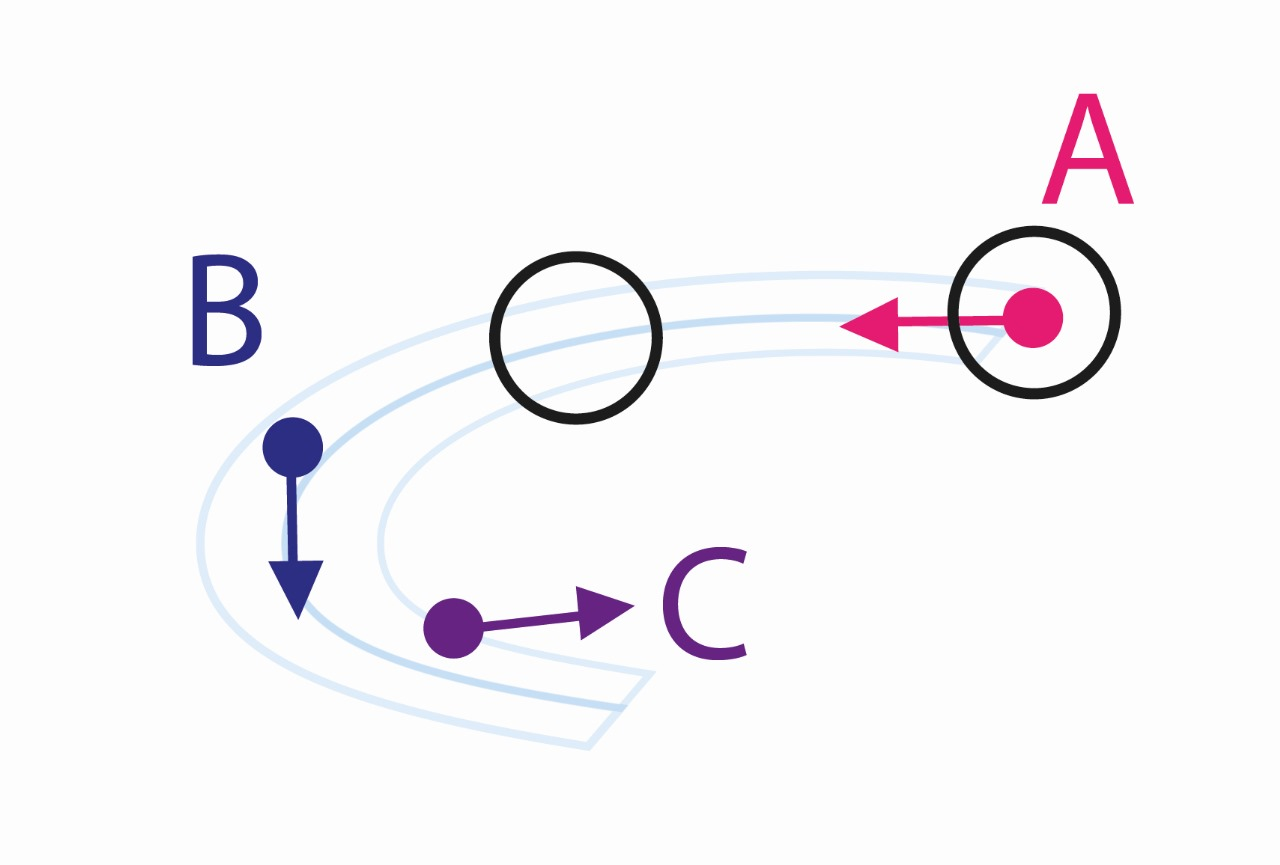
\includegraphics[width=0.6\linewidth]{Diagrama1.jpg}
    \caption{Posiciones de las partículas en donde se trackeó su trayectoria para cada corriente, representadas por los distintos colores, y las flechas representando sus trayectorias esperadas.}
\end{figure}
Para una corriente de 0.15A, obtuvimos las siguientes gráficas:

\begin{figure}[H]
    \centering
    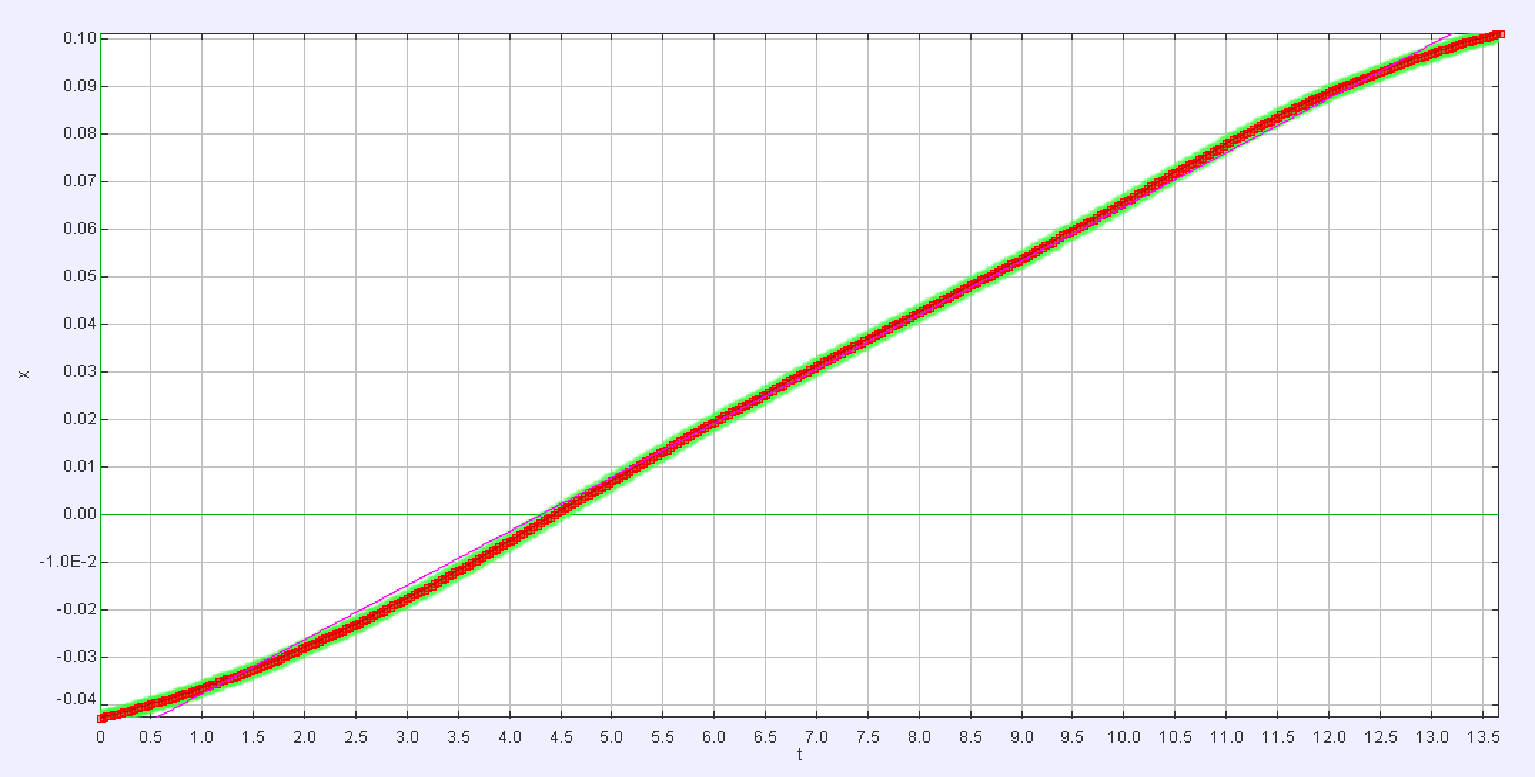
\includegraphics[width=0.8\linewidth]{Gráfica150mA_1.png}
    \caption{Gráfica de posición vs tiempo Para la partícula A. Con 0.15A}
\end{figure}
\begin{figure}[H]
    \centering
    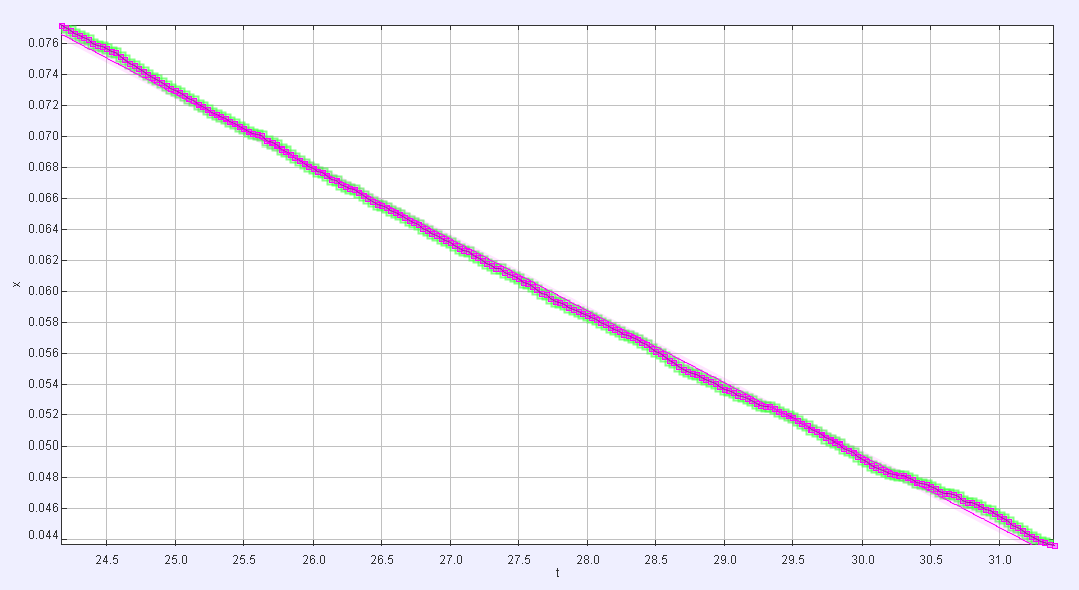
\includegraphics[width=0.8\linewidth]{Gráfica150mA_2.png}
    \caption{Gráfica de posición vs tiempo Para la partícula B. Con 0.15A}
\end{figure}
\begin{figure}[H]
    \centering
    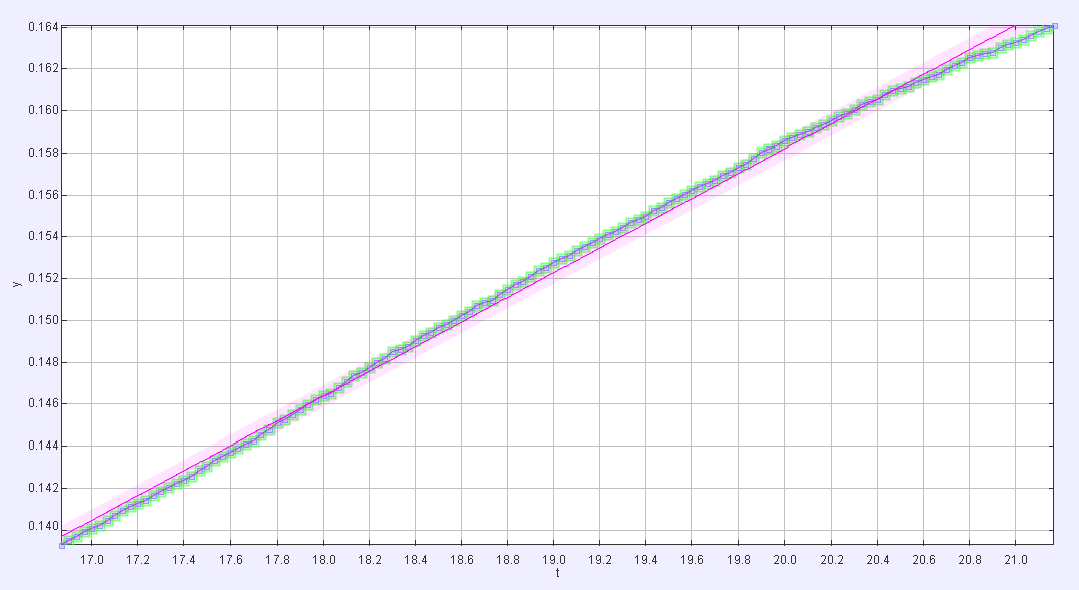
\includegraphics[width=0.8\linewidth]{Gráfica150mA_3.png}
    \caption{Gráfica de posición vs tiempo Para la partícula C. Con 0.15A}

\end{figure}
(Los datos de las posiciones superan las 400 columnas, así que se omitirán para no obstruir el análisis de los resultados, y se anexarán solo las tablas con las que se generaron las primeras 3 gráficas)
De estas gráficas, observamos una dependencia lineal de la posición en función del tiempo. Así, podemos obtener la velocidad del flujo en estos puntos, haciendo una regresión lineal , a partir de la relación $d=vt$, pues la velocidad estará dada por la pendiente de la gráfica.

\begin{table}[H]
\centering
\begin{tabular}{|l|l|l|l|}
\hline
\multicolumn{1}{|c|}{0.15A} & \multicolumn{1}{c|}{Partícula A}  & Partícula B                       & Partícula C                         \\ \hline
Velocidad (m/s)             & 0.0138 $\pm$ 0.00002 & 0.0047 $\pm$ 0.00001 & 0.00591 $\pm$ 0.000003 \\ \hline
\end{tabular}

\caption{Velocidad de las partículas A, B, C, representando la velocidad del flujo en esos puntos. Con una corriente de 0.15A}
\end{table}

Para una corriente de 0.30A tenemos las siguientes gráficas:
\begin{figure}[H]
    \centering
    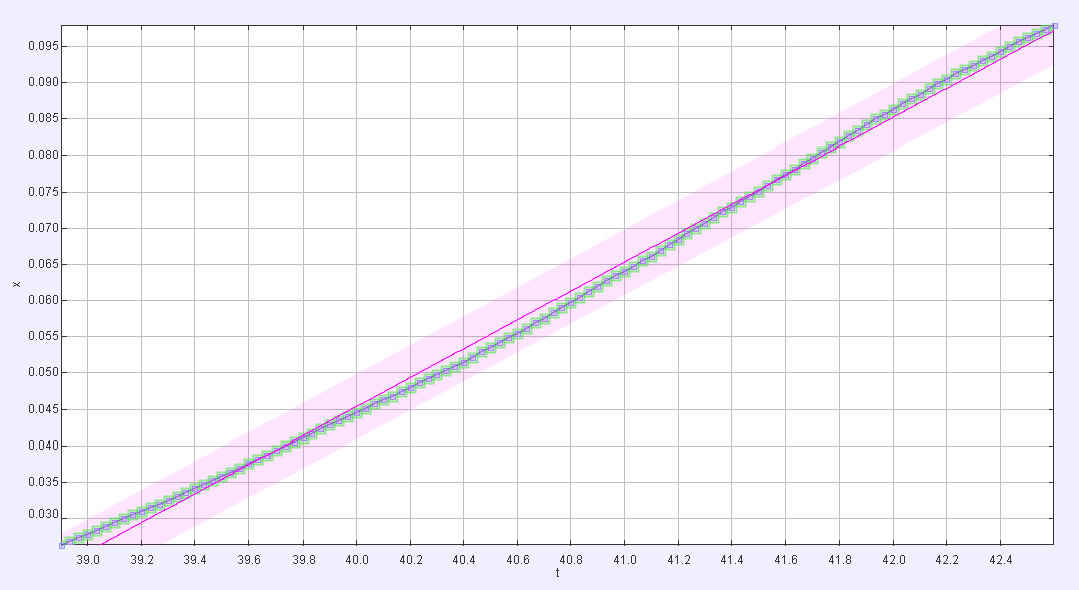
\includegraphics[width=0.7\linewidth]{Gráfica300mA_1.png}
    \caption{Gráfica de posición vs tiempo Para la partícula A. Con 0.30A}
\end{figure}
\begin{figure}[H]
    \centering
    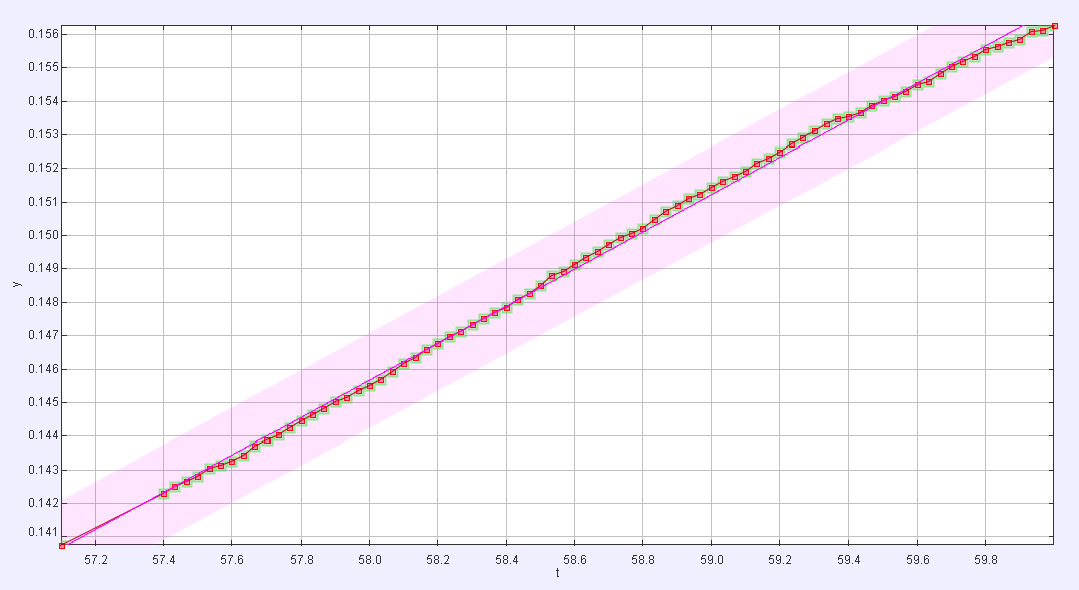
\includegraphics[width=0.7\linewidth]{Gráfica300mA_2.png}
    \caption{Gráfica de posición vs tiempo Para la partícula B. Con 0.30A}
\end{figure}
\begin{figure}[H]
    \centering
    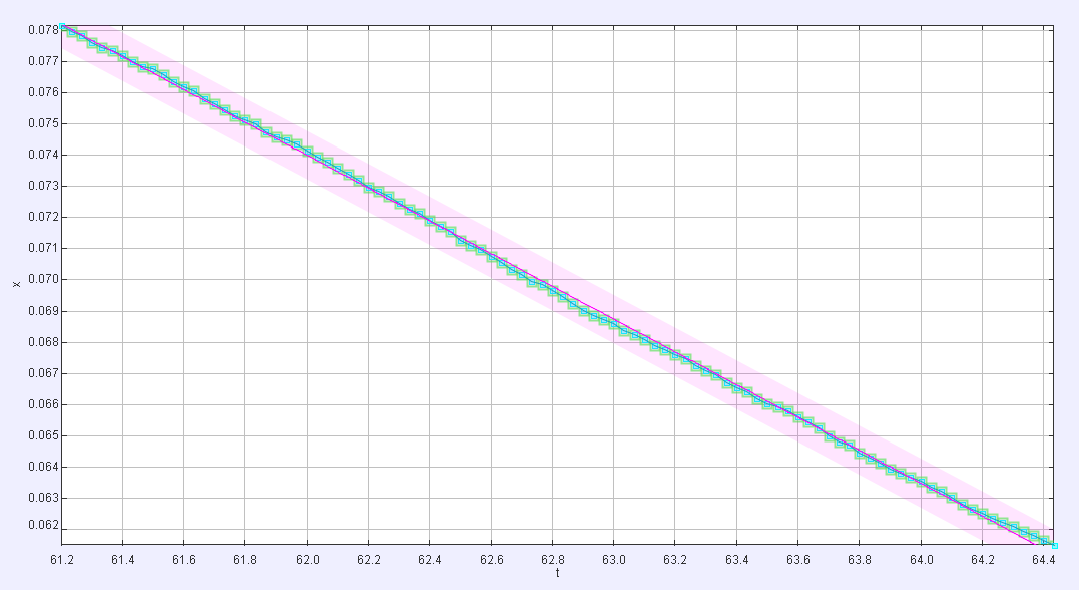
\includegraphics[width=0.7\linewidth]{Gráfica300mA_3.png}
    \caption{Gráfica de posición vs tiempo Para la partícula C. Con 0.30A}
\end{figure}

Y haciendo la regresión lineal obtenemos las velocidades:

\begin{table}[H]
\centering
\begin{tabular}{|l|l|l|l|}
\hline
\multicolumn{1}{|c|}{0.30A} & \multicolumn{1}{c|}{Partícula A}  & Partícula B                       & Partícula C                         \\ \hline
Velocidad (m/s)             & 0.0199 $\pm$ 0.00001 & 0.0055 $\pm$ 0.00002 & 0.00525 $\pm$ 0.000003 \\ \hline
\end{tabular}
\caption{Velocidad de las partículas A, B, C, representando la velocidad del flujo en esos puntos. Con una corriente de 0.30 A}
\end{table}

Para una corriente de 0.45A tenemos las siguientes gráficas:
\begin{figure}[H]
    \centering
    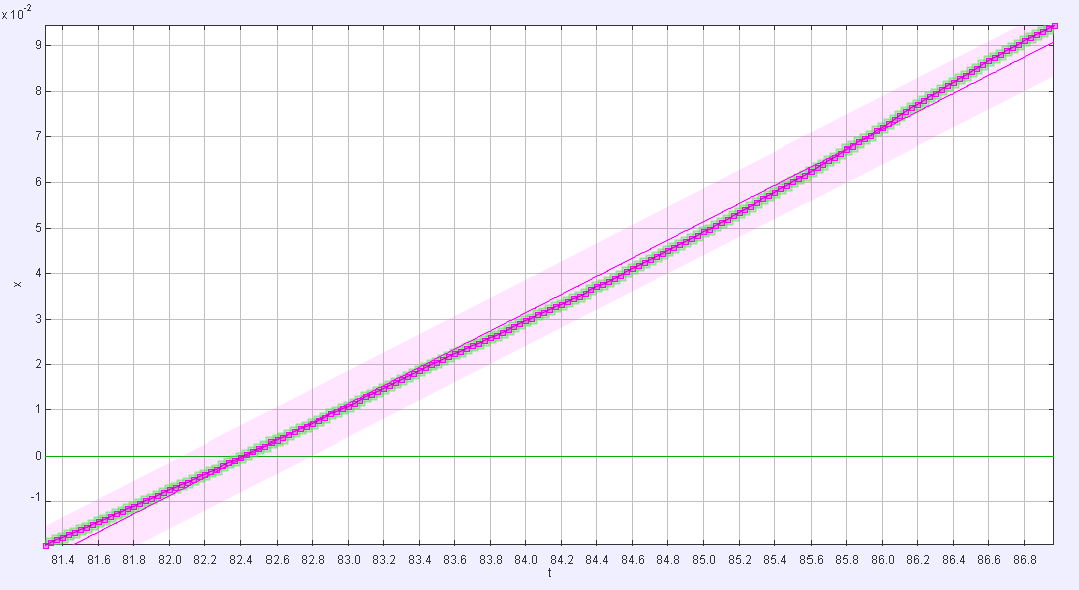
\includegraphics[width=0.7\linewidth]{Gráfica450mA_1.png}
    \caption{Gráfica de posición vs tiempo Para la partícula A. Con 0.45A}
\end{figure}
\begin{figure}[H]
    \centering
    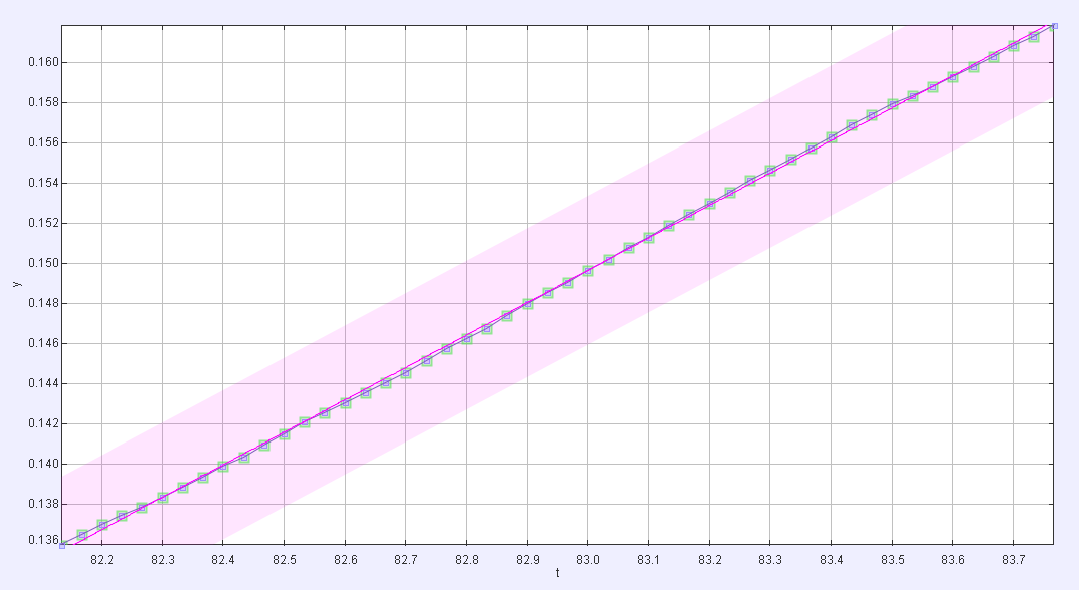
\includegraphics[width=0.7\linewidth]{Gráfica450mA_2.png}
    \caption{Gráfica de posición vs tiempo Para la partícula B. Con 0.45A}
\end{figure}
\begin{figure}[H]
    \centering
    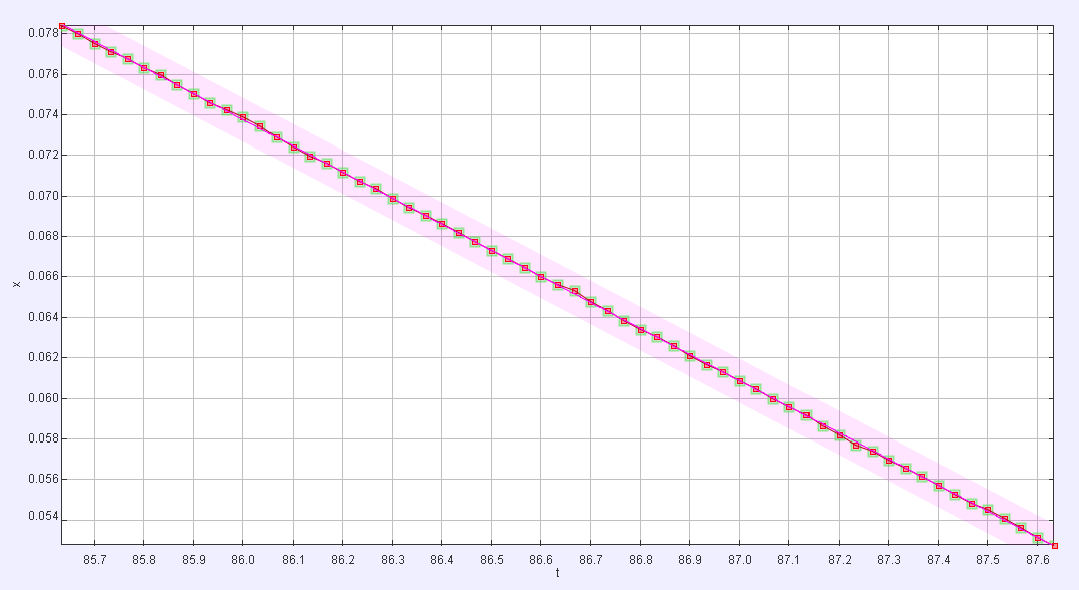
\includegraphics[width=0.7\linewidth]{Gráfica450mA_3.png}
    \caption{Gráfica de posición vs tiempo Para la partícula C. Con 0.45A}
\end{figure}
Y haciendo la regresión lineal obtenemos las velocidades:
\begin{table}[H]
\centering
\begin{tabular}{|l|l|l|l|}
\hline
\multicolumn{1}{|c|}{0.45A} & \multicolumn{1}{c|}{Partícula A}  & Partícula B                       & Partícula C                        \\ \hline
Velocidad (m/s)             & 0.02004 $\pm$ 0.0009 & 0.01615 $\pm$ 0.0002 & 0.01288 $\pm$ 0.00001 \\ \hline
\end{tabular}
\caption{Velocidad de las partículas A, B, C, representando la velocidad del flujo en esos puntos. Con una corriente de 0.45 A}
\end{table}

\subsection{Parte cualitativa}
\subsubsection{Arreglo un imán}
\begin{figure}[H]
    \centering
    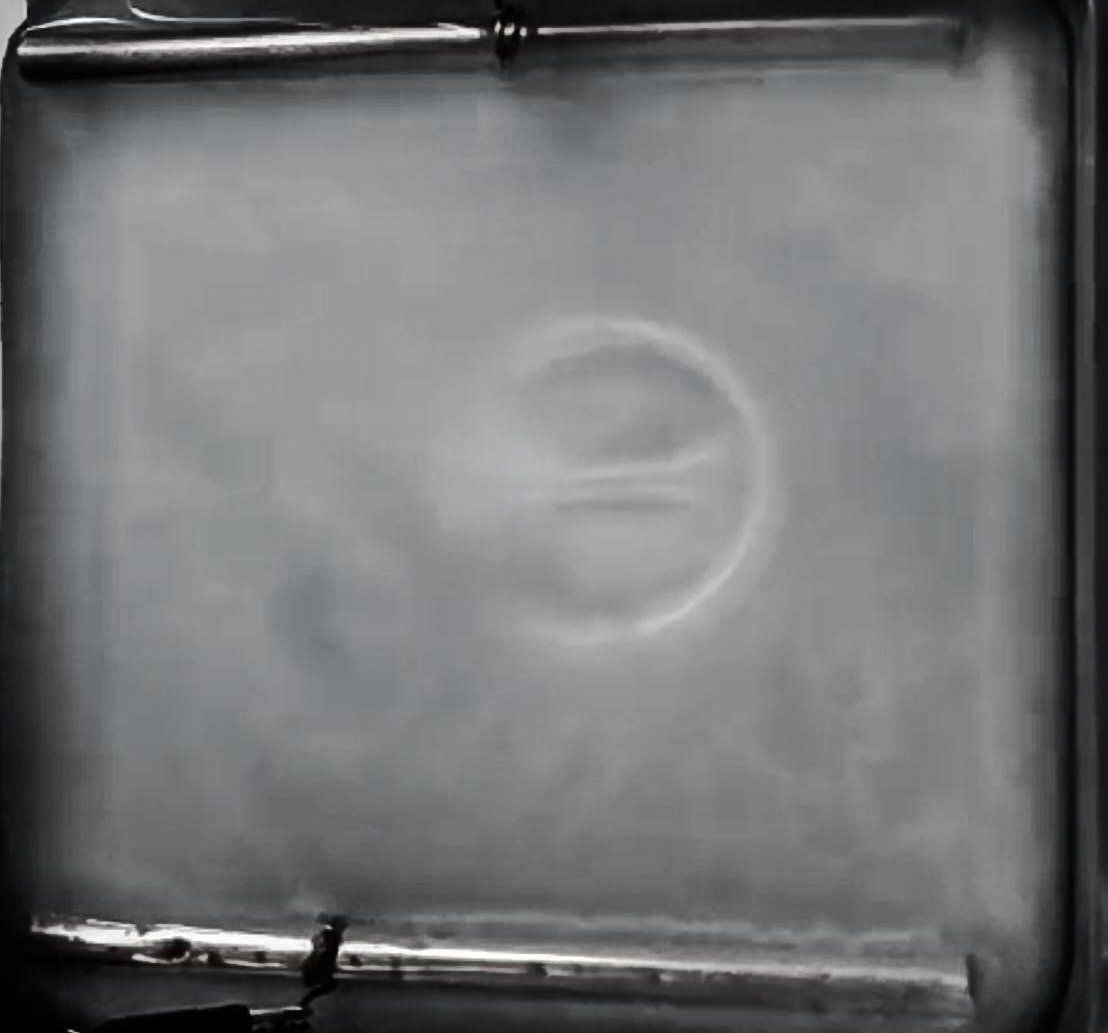
\includegraphics[width=0.5\linewidth]{1iman1.png}
    \caption{Primeros instantes del arreglo de un imán}
    \label{fig:enter-label}
\end{figure}
Hemos colocado el imán con un polo aleatorio hacia arriba, en los primeros instantes al suministrarle 150mA de corriente eléctrica, el fluido reoscópico describió un \textit{brazo} o \textit{orejita} hacia la derecha. Al pasar 7 segundos incrementó su magnitud como se observa en la Figura 12.

\begin{figure}[H]
    \centering
    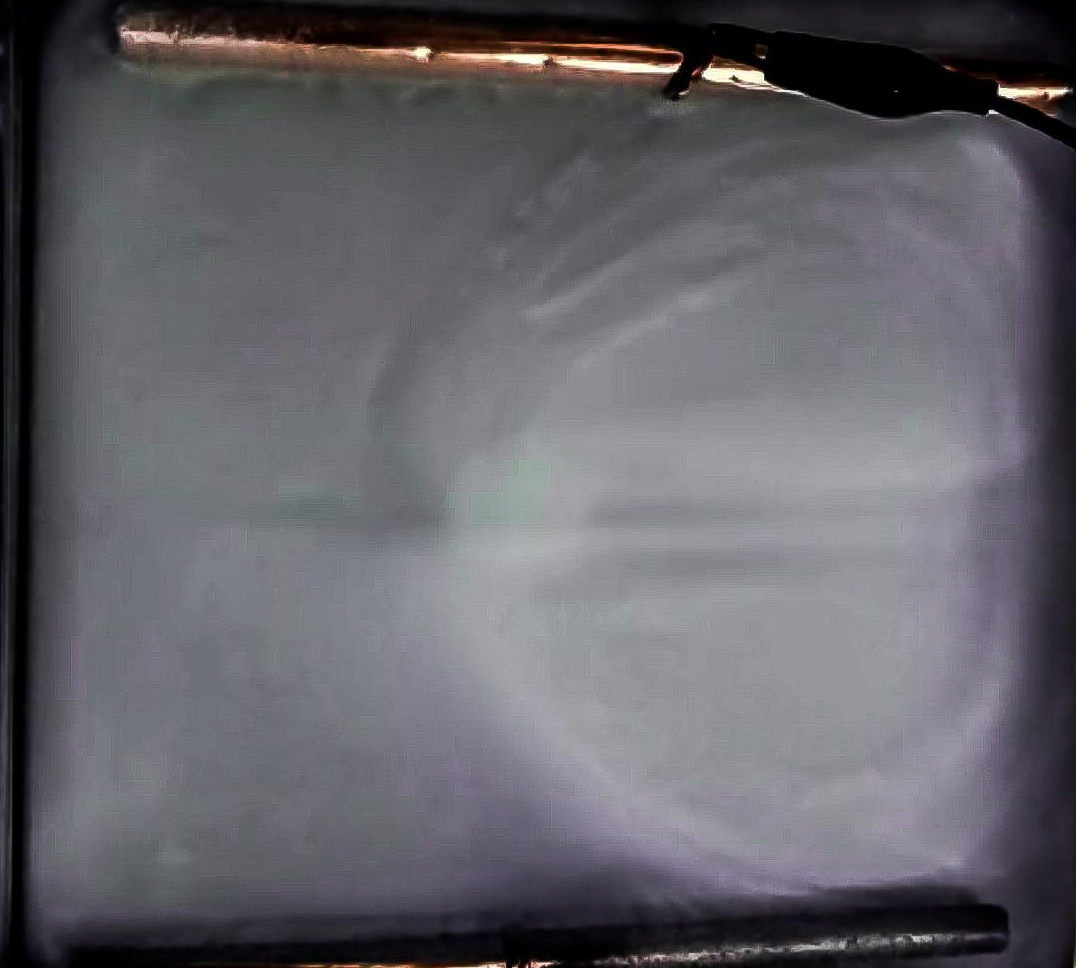
\includegraphics[width=0.5\linewidth]{1iman2.png}
    \caption{7 segundos posteriormente a la suministración de corriente a un imán}
    \label{fig:enter-label}
\end{figure}

Posterior a estos 7 segundos el fluído mantuvo una forma exactamente igual; ahora repetimos el experimento con 300mA de corriente eléctrica suministrada, el resultado en fotos fue exactamente el mismo por lo que no se adjuntarán imágenes innecesarias, sin embargo la velocidad del fluído era considerablemente más rápida por lo que lo observado en Figura 12 fue más rápido de verse; finalmente se hizo con 450mA y nuevamente obtuvimos lo mismo, pero con una velocidad increíblemente rápida. \\

Ahora bien, al invertir el polo del imán y repetir el experimento, fue interesante ver que es exactamente igual en figuras descritas y velocidad al primer caso de Figura 11 pero con apertura a la izquierda. Como se espera, también experimentó los mismos cambios de velocidades al incrementar progresivamente la corriente eléctrica de $150mA \rightarrow 300mA \rightarrow 450mA$.


\subsubsection{Arreglo pareja de imanes}

Es aquí en donde tenemos arreglos más interesantes, llámese al patrón descrito por un solo imán con forma de una \textit{"orejita de pan"} como el \textbf{caso elemental}. Nuestro primer análisis será para cuando nuestros dos imanes están colocados con el mismo polo hacia arriba.

Mírese en la siguiente imagen los primeros instantes (se denomina en este estudio como primeros instantes una vez suministrada la corriente eléctrica) del caso para dos imanes iguales, es tan rápido el lapso en el que la traza del flujo de ambos imanes se une que no da tiempo de tintarlos y mostrar lo que cada imán individualmente produce en el segundo 1. Observamos que cuando tenemos esta disposición de imanes es como si tuvieramos el caso elemental superpuesto como si de un sticker se tratase, pero al transcurrir poco más de un segundo al apuntar ambos al mismo lado la pintura describe una línea horizontal que une ambos imanes y actua como el caso elemental alargado elípticamente.

\begin{figure}[H]
    \centering
    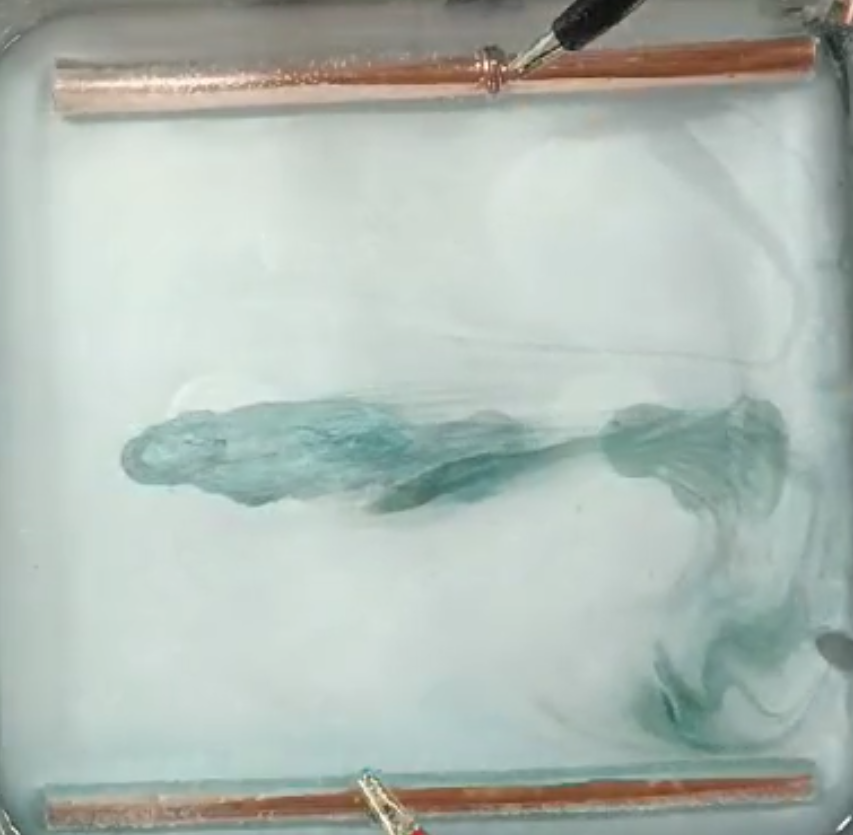
\includegraphics[width=0.5\linewidth]{2imanes=1.png}
    \caption{Primeros instantes del arreglo de dos imanes de polos iguales}
    \label{fig:enter-label}
\end{figure}

Ahora véase 4 segundos posterior al suministro de corriente, el patrón descrito es demasiado fuerte, como si hubiésemos incrementado la imagen del imán del caso elemental. 

\begin{figure}[H]
    \centering
    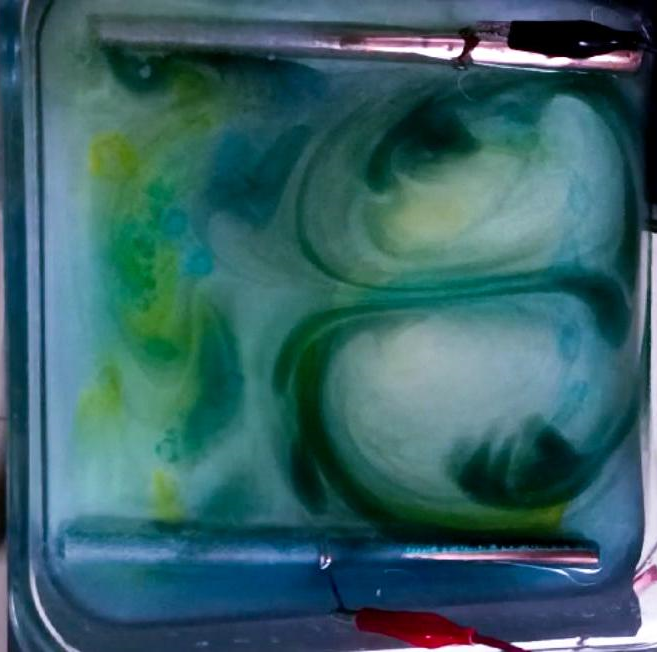
\includegraphics[width=0.5\linewidth]{2imanes=.png}
    \caption{4 primeros segundos del arreglo de dos imanes de polos iguales}
    \label{fig:enter-label}
\end{figure}

Finalmente al transcurrir 8 segundos mantiene un patrón uniforme demasiado prominente, es interesante mencionar que notamos unas pequeñas colitas en el lado opuesto al \textit{brazo} llegado a este punto.

\begin{figure}[H]
    \centering
    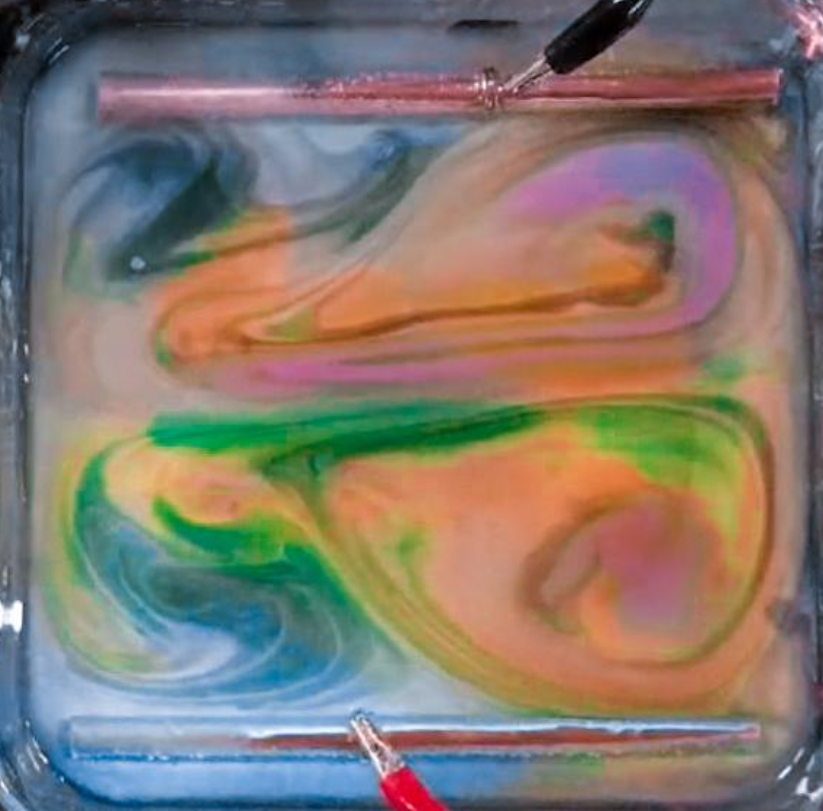
\includegraphics[width=0.5\linewidth]{2imanes=2.png}
    \caption{Estado pasado 8 segundos del arreglo de dos imanes de polos iguales}
    \label{fig:enter-label}
\end{figure}

Probamos qué sucedía para los casos que se suministra 300mA y 450mA, nuevamente el fluído incrementó proporcionalmente su velocidad y por ende su tiempo que le toma en llegar a lo que denominamos \textbf{patrón de equilibrio}; para el caso con ambos imanes con el polo invertido respecto a la prueba anterior ocurrió exactamente lo mismo pero con la superposición del caso elemental mirando hacia la izquierda, asímismo el comportamiento con el incremento de corriente sigue causando un incremento en la velocidad.\\

Ahora obsérvese el caso para ambos imanes con disposición de polos diferentes, es gracioso y retroalimentador observar que si estos no se alinean perfectamente con el centro ocurre lo siguiente.

\begin{figure}[H]
    \centering
    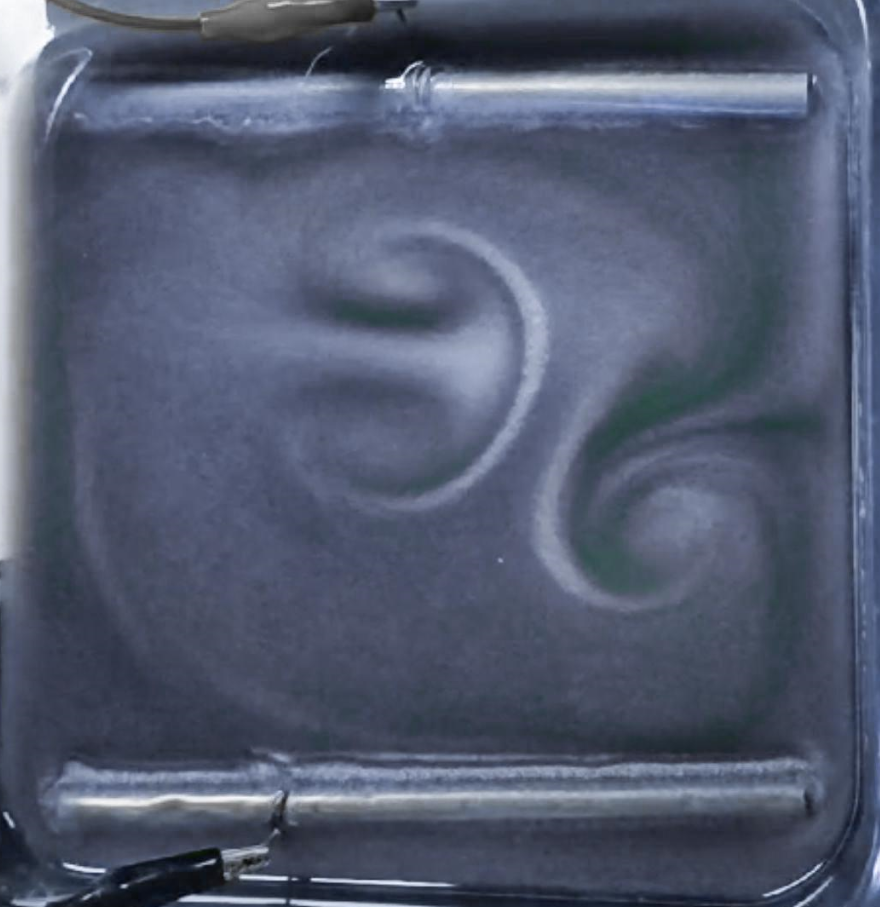
\includegraphics[width=0.5\linewidth]{2imanesdif.png}
    \caption{Primeros instantes de arreglo geométricamente irregular de dos imanes con polos contrarios}
    \label{fig:enter-label}
\end{figure}

Nuevamente miramos que el caso elemental de acuerdo al polo que esté mirando hacia arriba de cada imán simplemente se superpone visualmente encima de cada uno de ellos, respetando la dirección a la que apuntaría si fuese un solo imán, repetimos el experimento con los imanes bien alineados y la imagen es igual que Figura 16 pero con la colisión perfectamente centrada. Ahora hicimos el mismo arreglo de imanes de polo diferente pero intercambiándolos de lugar, esperando que no haya una colisión, el resultado fue satisfactorio y puede usted observarlo en la siguiente imagen.

\begin{figure}[H]
    \centering
    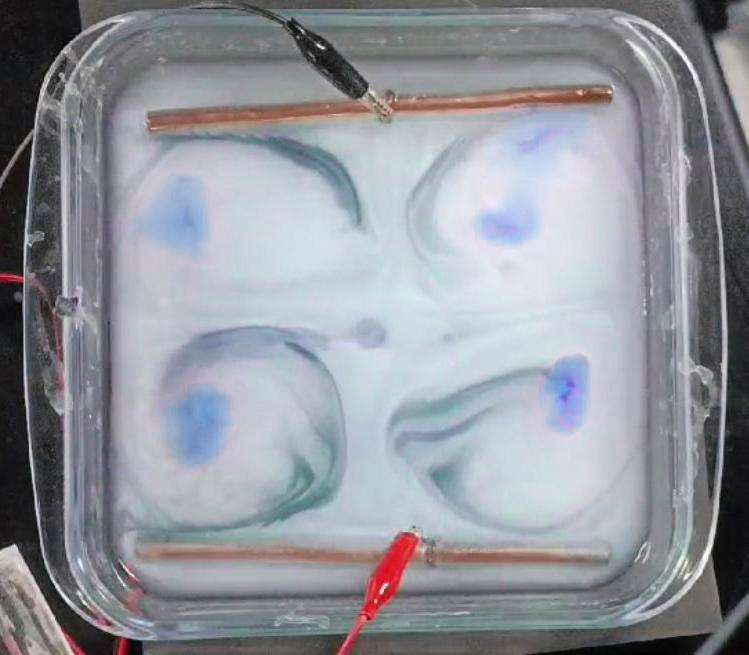
\includegraphics[width=0.5\linewidth]{2imanesdiff.jpg}
    \caption{Primeros instantes del arreglo de dos imanes de polos diferentes}
    \label{fig:enter-label}
\end{figure}

Pero algo extraño sucedió pasando 8 segundos, se creó el siguiente patrón.

\begin{figure}[H]
    \centering
    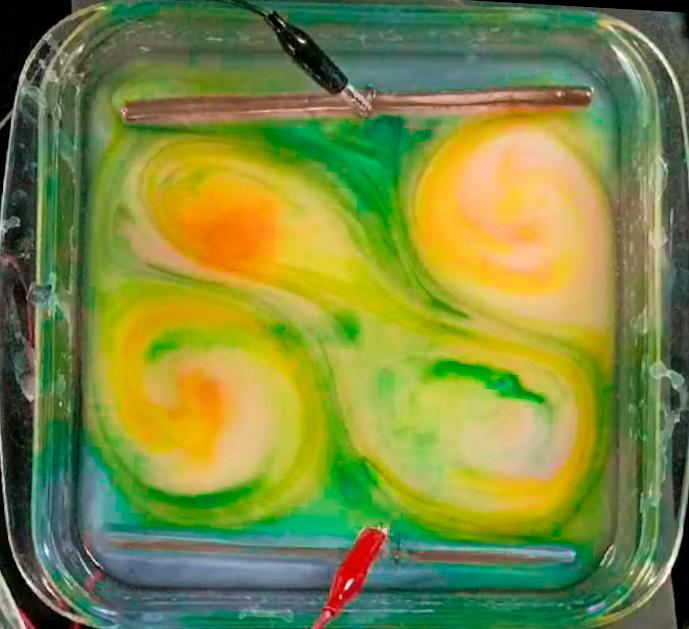
\includegraphics[width=0.5\linewidth]{2imanesdiferentes.jpg}
    \caption{Estado de equilibrio de dos imanes de polos diferentes}
    \label{fig:enter-label}
\end{figure}

Dos lados diagonalmente opuestos de orejitas que aparentemente son ajenas interactuaron entre sí, explorando causas vimos que los imanes a pesar de estar milimétricamente centrados, presentaban errores en su geometría respecto al centro, los movimos muy ligeramente y la diagonal que interactua pasó a ser la otra. Hemos intentado preservar ambas orejitas sin interactuar entre sí, sin embargo, el arreglo debido a la potencia de los imanes y el tamaño del refractario es muy sensible por lo que ha sido imposible, sugerimos en futuros estudios explorar si es más sencillo con un refractario de mayor tamaño así como mayor separación entre los imanes; a partir de aquí omitiré mencionar qué sucede al incrementar la corriente eléctrica pues, \textit{adelanto}, en todos se sigue que a mayor intensidad de corriente mayor es la velocidad presente en cada partícula fluída.

\subsubsection{Arreglo azaroso de imanes}

Aquí experimentamos con 4 imanes en este caso los de 12mm de diámetro como se observa en la siguiente imagen.

\begin{figure}[H]
    \centering
    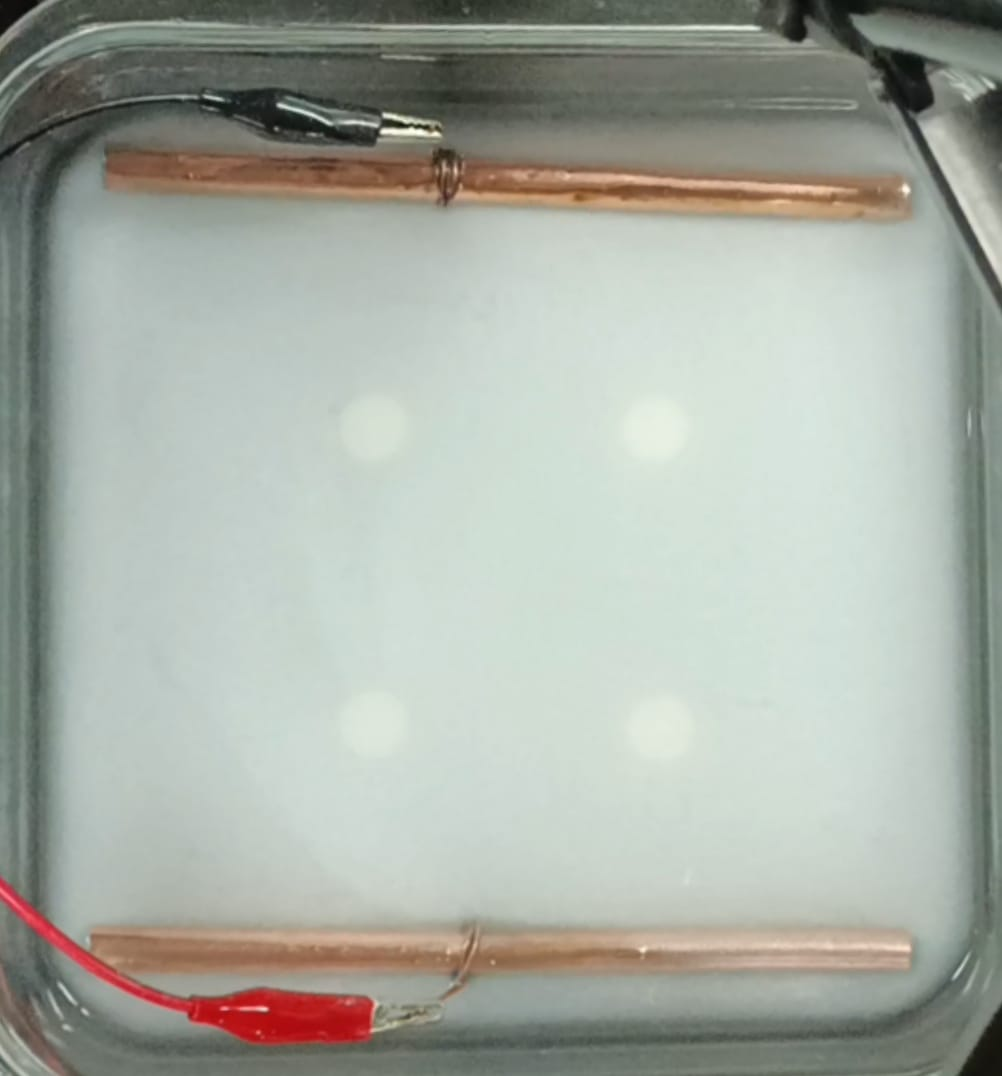
\includegraphics[width=0.5\linewidth]{4imanes0.jpg}
    \caption{Arreglo para 4 imanes}
    \label{fig:enter-label}
\end{figure}

Para nuestro primer experimento y con lo que hemos aprendido en este camino, observamos qué pasa cuando todos los imanes tienen su polo orientado hacia arriba diferente a su lateral inmediato, como si un arreglo de ajedrez 2x2 se tratase. Dada la naturaleza de este arreglo esperamos que ya sea en la zona superior o inferior, una "\textit{pareja de fluidos}" se aleje entre sí, como el caso elemental donde (tomar con pinzas la expresión) cada fluido del imán apunta hacia una dirección opuesta, mientras que la otra pareja de imanes análogo a lo visto en la sección 3.2.2 intercambiando lugares del imán, simplemente colisionarán.

\begin{figure}[H]
    \centering
    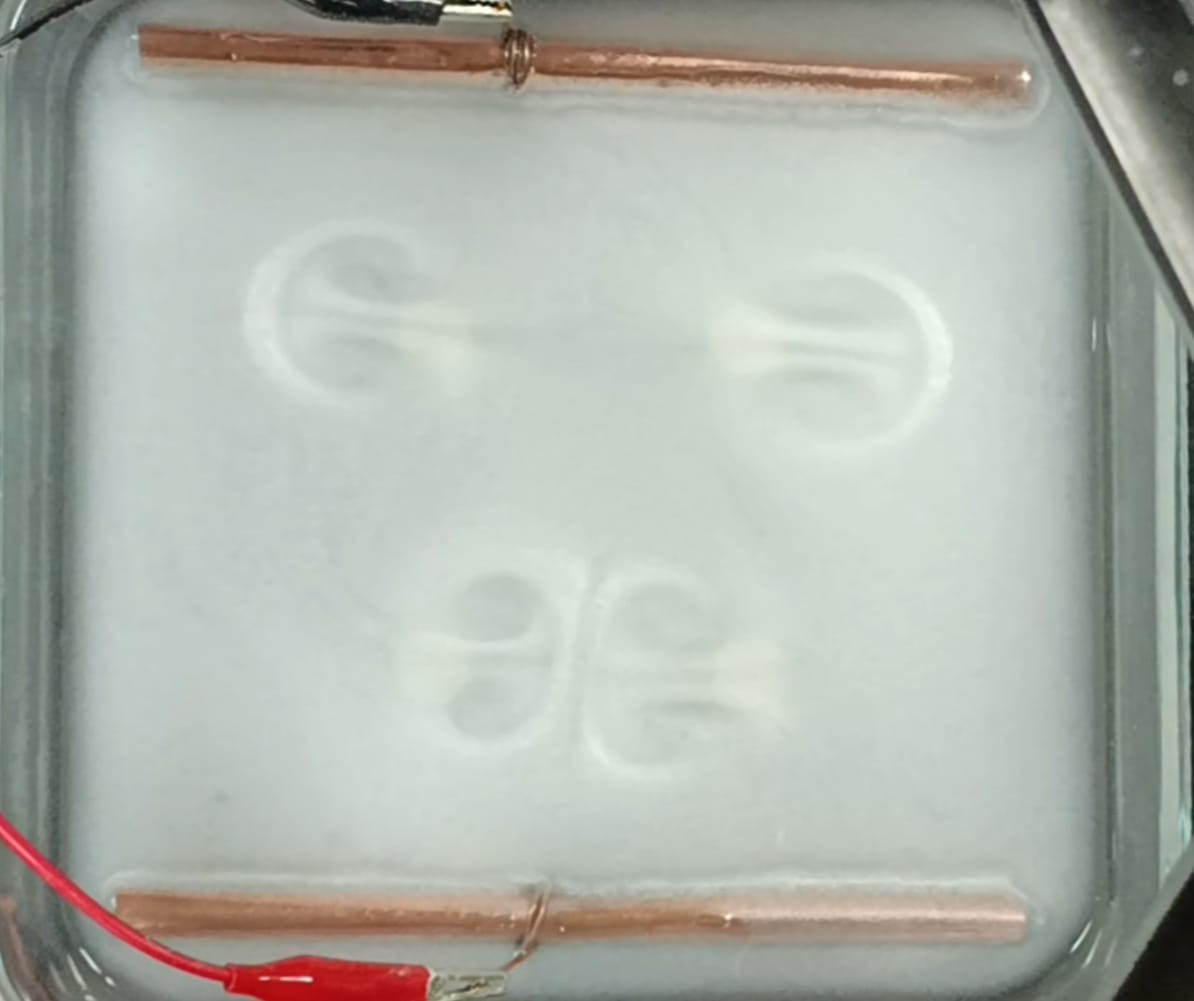
\includegraphics[width=0.5\linewidth]{4imanesdiftodos.jpg}
    \caption{Primeros instantes de arreglo para 4 imanes de polos opuestos respecto a su lateral inmediato}
    \label{fig:enter-label}
\end{figure}

Es visualmente muy agradable a la vista, por ahora, cómo tenemos una superposición de 4 casos elementales que respetan la orientación de su polo. No obstante, hemos reportado un comportamiento indescriptible al transcurrir 6 segundos vease en la siguiente imagen.

\begin{figure}[H]
    \centering
    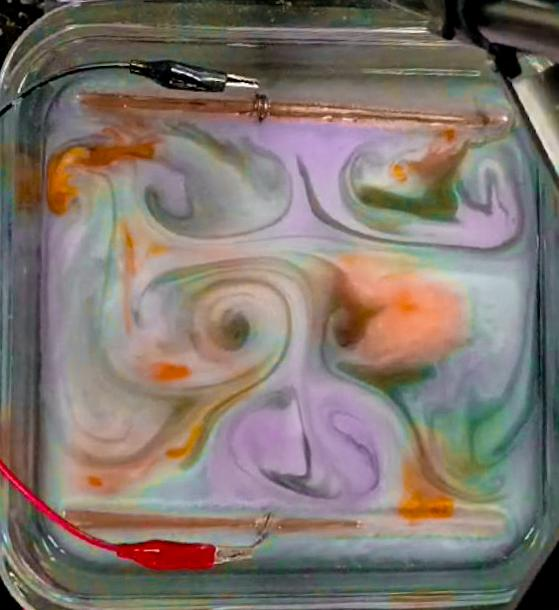
\includegraphics[width=0.5\linewidth]{4imanesindesc1.jpg}
    \caption{Mismo arreglo transcurridos 6 segundos respecto al suministro de corriente}
    \label{fig:enter-label}
\end{figure}

Y se vuelve peor 4 segundos más después.

\begin{figure}[H]
    \centering
    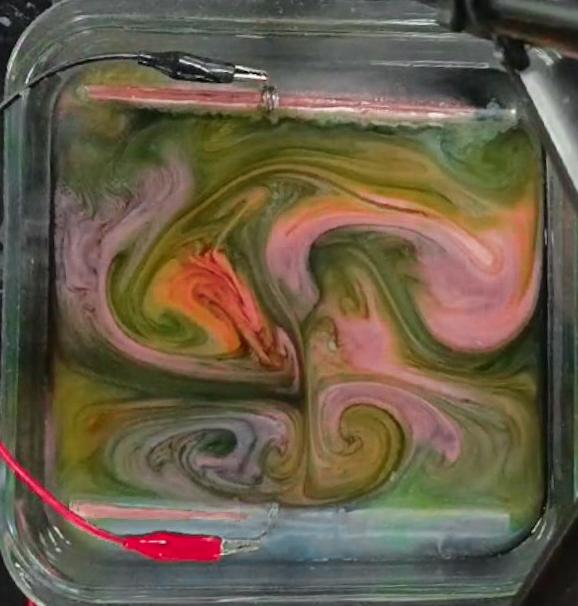
\includegraphics[width=0.5\linewidth]{4imanesindesc2.jpg}
    \caption{Mismo arreglo transcurridos 10 segundos respecto al suministro de corriente}
    \label{fig:enter-label}
\end{figure}

En este caso, no existió un patrón de equilibrio, siempre estuvo es una constante distorsión aún transcurriendo un minuto completo; el caso para todos los imanes con misma disposición como es esperable solo superpuso 4 casos elementales por encima de cada imán con misma dirección, sin embargo, contrario a lo que se esperaría en un inicio fue el caso más desastrozo de todos al transcurrir el tiempo, este fue estudiado durante un mayor tiempo y después de 5 minutos jamás llegó a un patrón elemental, mírese en la imagen de a continuación.

\begin{figure}[H]
    \centering
    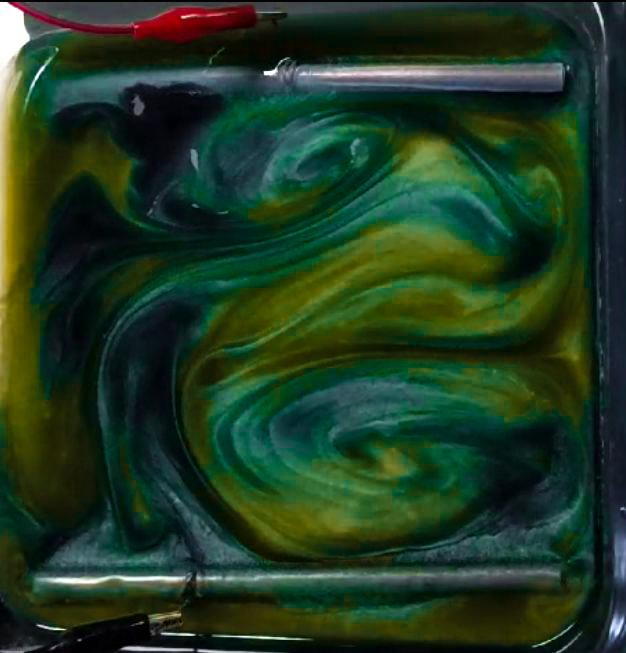
\includegraphics[width=0.5\linewidth]{4imanes=s.jpg}
    \caption{Arreglo de 4 imanes con misma disposición al transcurrir 20 segundos respecto al suministro de corriente}
    \label{fig:enter-label}
\end{figure}

Creemos que los sutiles errores en la geometría de la disposición cuadrada de los imanes se debe a la superposición de campos, lo cual al tener un campo demasiado prominente se refleja como si estos errores geométricos fueran bastante más grandes.

\section{Conclusiones}
Podemos observar de las tablas de velocidades que hay una relación proporcional entre la velocidad y el aperaje suministrado. Además, en los puntos cercanos al imán, la velocidad registrada es mayor. En general, el presente estudio en magnetohidrodinámica ha revelado cómo las configuraciones geométricas y la polaridad de imanes de neodimio interactúan con un fluido reoscópico conductor bajo la influencia de corrientes eléctricas. El análisis experimental detallado de arreglos desde un solo imán hasta configuraciones multimodales de cuatro imanes demuestra que los patrones observados en el flujo son sensibles a factores como la intensidad de corriente, la orientación de los polos y las propiedades geométricas del sistema.

En configuraciones simples, como un solo imán o pares de imanes, los resultados confirmaron patrones predecibles y repetibles, destacando la influencia directa de la polaridad y la corriente en la velocidad y dirección del flujo. Sin embargo, al explorar arreglos más complejos, como cuatro imanes en disposiciones alternadas o uniformes, emergieron dinámicas caóticas y transiciones inesperadas en los patrones de flujo. Estas anomalías sugieren una amplificación de errores geométricos y la superposición no lineal de campos magnéticos, generando comportamientos fuera de equilibrio que no estabilizan incluso tras tiempos prolongados.

Estos hallazgos subrayan la importancia de la precisión geométrica y la alineación en experimentos magnetohidrodinámicos complejos. Además, abren la puerta a futuras investigaciones para comprender mejor las transiciones entre regímenes de equilibrio y caos en sistemas similares. Ampliar el tamaño del recipiente o la separación de los imanes podría mitigar las interacciones indeseadas y permitir un estudio más controlado de los patrones de flujo. Este trabajo no solo contribuye al conocimiento fundamental de la magnetohidrodinámica, sino que también establece una base para aplicaciones prácticas en control de fluidos y diseño de sistemas electromagnéticos avanzados.
\newpage
\noindent {\bf Declaración de contribución de los autores}\\ 

Iván Bautista Alvarado$^1$ y Andrés López González$^1$ hemos realizado tanto el apartado escrito como el análisis de manera colectiva siendo una participación del 100\% por parte de ambos y no solo una repartición.\\ 

\section{Anexo}
Foto de la disposicion de las basuritas usadas para trackear las posiciones.

\begin{figure}[H]
    \centering
    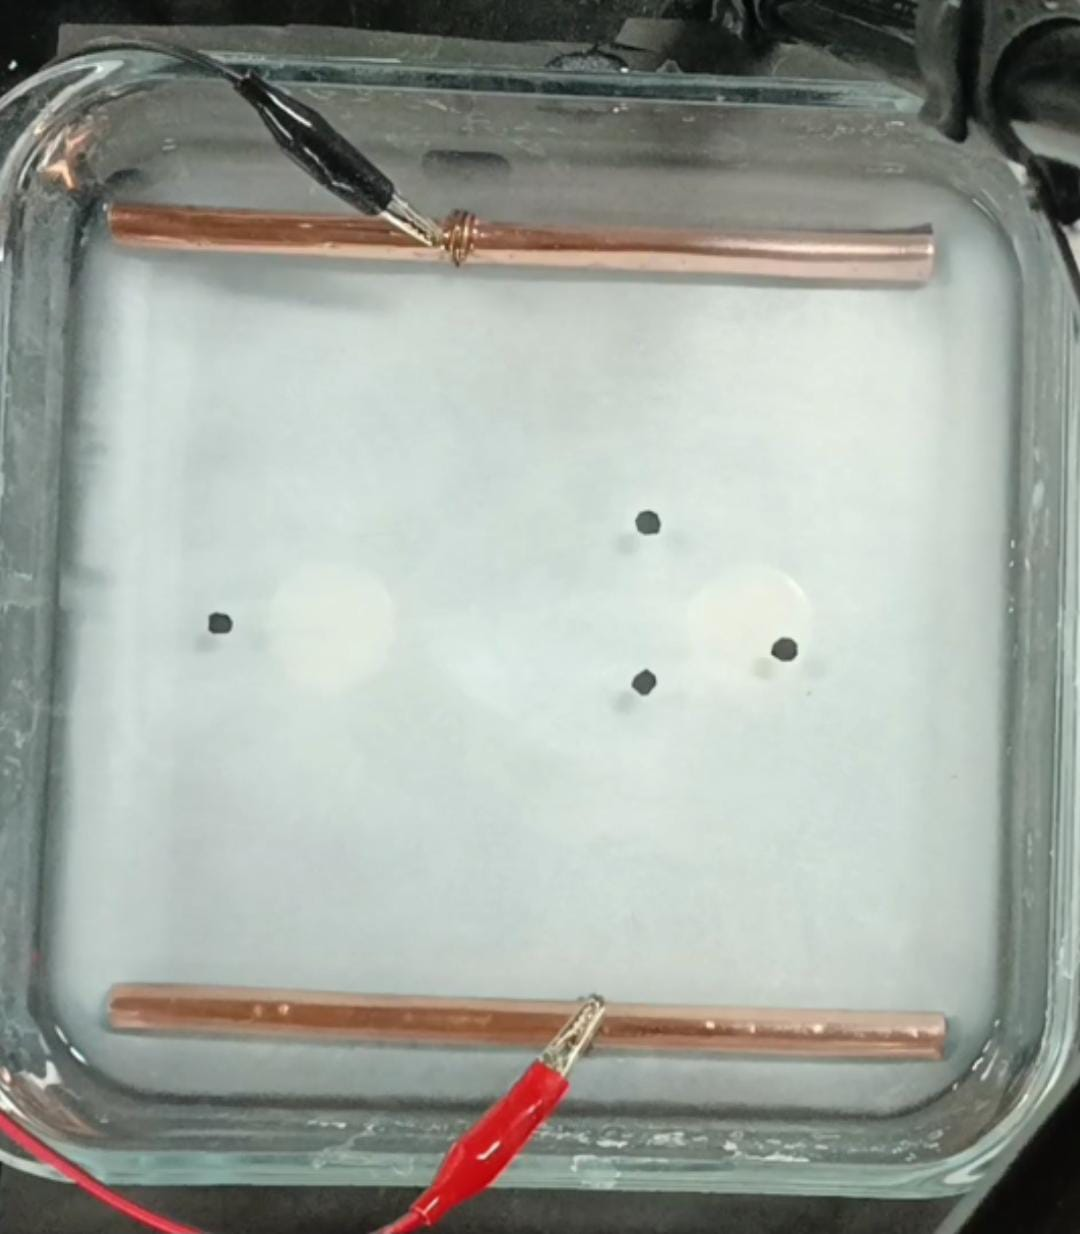
\includegraphics[width=0.6\linewidth]{FotoTrakeo.jpg}
    \caption{Imagen de las basuritas siguiendo el flujo del fluido}
\end{figure}\\

A continuación se anexan tres tablas de datos obtenidos para las gráficas de posición vs tiempo.

\begin{longtable}[c]{|c|c|cccccc}
\hline
Partícula\_A  &           & \multicolumn{1}{c|}{} & \multicolumn{1}{c|}{Partícula\_B} & \multicolumn{1}{c|}{}      & \multicolumn{1}{c|}{} & \multicolumn{1}{c|}{Partícula\_C} & \multicolumn{1}{c|}{}         \\ \hline
\endfirsthead
%
\endhead
%
t        & x         & \multicolumn{1}{c|}{} & \multicolumn{1}{c|}{t}       & \multicolumn{1}{c|}{y}     & \multicolumn{1}{c|}{} & \multicolumn{1}{c|}{t}       & \multicolumn{1}{c|}{x}        \\ \hline
0.000    & -4.273E-2 & \multicolumn{1}{c|}{} & \multicolumn{1}{c|}{16.90}   & \multicolumn{1}{c|}{0.139} & \multicolumn{1}{c|}{} & \multicolumn{1}{c|}{24.17}   & \multicolumn{1}{c|}{7.719E-2} \\ \hline
3.333E-2 & -4.251E-2 & \multicolumn{1}{c|}{} & \multicolumn{1}{c|}{16.93}   & \multicolumn{1}{c|}{0.140} & \multicolumn{1}{c|}{} & \multicolumn{1}{c|}{24.20}   & \multicolumn{1}{c|}{7.705E-2} \\ \hline
6.667E-2 & -4.238E-2 & \multicolumn{1}{c|}{} & \multicolumn{1}{c|}{16.97}   & \multicolumn{1}{c|}{0.140} & \multicolumn{1}{c|}{} & \multicolumn{1}{c|}{24.23}   & \multicolumn{1}{c|}{7.684E-2} \\ \hline
0.100    & -4.217E-2 & \multicolumn{1}{c|}{} & \multicolumn{1}{c|}{17.00}   & \multicolumn{1}{c|}{0.140} & \multicolumn{1}{c|}{} & \multicolumn{1}{c|}{24.27}   & \multicolumn{1}{c|}{7.663E-2} \\ \hline
0.133    & -4.208E-2 & \multicolumn{1}{c|}{} & \multicolumn{1}{c|}{17.03}   & \multicolumn{1}{c|}{0.140} & \multicolumn{1}{c|}{} & \multicolumn{1}{c|}{24.30}   & \multicolumn{1}{c|}{7.649E-2} \\ \hline
0.167    & -4.193E-2 & \multicolumn{1}{c|}{} & \multicolumn{1}{c|}{17.07}   & \multicolumn{1}{c|}{0.140} & \multicolumn{1}{c|}{} & \multicolumn{1}{c|}{24.33}   & \multicolumn{1}{c|}{7.635E-2} \\ \hline
0.200    & -4.171E-2 & \multicolumn{1}{c|}{} & \multicolumn{1}{c|}{17.10}   & \multicolumn{1}{c|}{0.141} & \multicolumn{1}{c|}{} & \multicolumn{1}{c|}{24.37}   & \multicolumn{1}{c|}{7.622E-2} \\ \hline
0.233    & -4.153E-2 & \multicolumn{1}{c|}{} & \multicolumn{1}{c|}{17.13}   & \multicolumn{1}{c|}{0.141} & \multicolumn{1}{c|}{} & \multicolumn{1}{c|}{24.40}   & \multicolumn{1}{c|}{7.602E-2} \\ \hline
0.267    & -4.135E-2 & \multicolumn{1}{c|}{} & \multicolumn{1}{c|}{17.17}   & \multicolumn{1}{c|}{0.141} & \multicolumn{1}{c|}{} & \multicolumn{1}{c|}{24.43}   & \multicolumn{1}{c|}{7.586E-2} \\ \hline
0.300    & -4.119E-2 & \multicolumn{1}{c|}{} & \multicolumn{1}{c|}{17.20}   & \multicolumn{1}{c|}{0.141} & \multicolumn{1}{c|}{} & \multicolumn{1}{c|}{24.47}   & \multicolumn{1}{c|}{7.577E-2} \\ \hline
0.333    & -4.097E-2 & \multicolumn{1}{c|}{} & \multicolumn{1}{c|}{17.23}   & \multicolumn{1}{c|}{0.141} & \multicolumn{1}{c|}{} & \multicolumn{1}{c|}{24.50}   & \multicolumn{1}{c|}{7.565E-2} \\ \hline
0.367    & -4.071E-2 & \multicolumn{1}{c|}{} & \multicolumn{1}{c|}{17.27}   & \multicolumn{1}{c|}{0.142} & \multicolumn{1}{c|}{} & \multicolumn{1}{c|}{24.53}   & \multicolumn{1}{c|}{7.546E-2} \\ \hline
0.400    & -4.045E-2 & \multicolumn{1}{c|}{} & \multicolumn{1}{c|}{17.30}   & \multicolumn{1}{c|}{0.142} & \multicolumn{1}{c|}{} & \multicolumn{1}{c|}{24.57}   & \multicolumn{1}{c|}{7.538E-2} \\ \hline
0.433    & -4.023E-2 & \multicolumn{1}{c|}{} & \multicolumn{1}{c|}{17.33}   & \multicolumn{1}{c|}{0.142} & \multicolumn{1}{c|}{} & \multicolumn{1}{c|}{24.60}   & \multicolumn{1}{c|}{7.517E-2} \\ \hline
0.467    & -4.004E-2 & \multicolumn{1}{c|}{} & \multicolumn{1}{c|}{17.37}   & \multicolumn{1}{c|}{0.142} & \multicolumn{1}{c|}{} & \multicolumn{1}{c|}{24.63}   & \multicolumn{1}{c|}{7.495E-2} \\ \hline
0.500    & -3.985E-2 & \multicolumn{1}{c|}{} & \multicolumn{1}{c|}{17.40}   & \multicolumn{1}{c|}{0.142} & \multicolumn{1}{c|}{} & \multicolumn{1}{c|}{24.67}   & \multicolumn{1}{c|}{7.472E-2} \\ \hline
0.533    & -3.965E-2 & \multicolumn{1}{c|}{} & \multicolumn{1}{c|}{17.43}   & \multicolumn{1}{c|}{0.143} & \multicolumn{1}{c|}{} & \multicolumn{1}{c|}{24.70}   & \multicolumn{1}{c|}{7.458E-2} \\ \hline
0.567    & -3.947E-2 & \multicolumn{1}{c|}{} & \multicolumn{1}{c|}{17.47}   & \multicolumn{1}{c|}{0.143} & \multicolumn{1}{c|}{} & \multicolumn{1}{c|}{24.73}   & \multicolumn{1}{c|}{7.436E-2} \\ \hline
0.600    & -3.920E-2 & \multicolumn{1}{c|}{} & \multicolumn{1}{c|}{17.50}   & \multicolumn{1}{c|}{0.143} & \multicolumn{1}{c|}{} & \multicolumn{1}{c|}{24.77}   & \multicolumn{1}{c|}{7.415E-2} \\ \hline
0.633    & -3.900E-2 & \multicolumn{1}{c|}{} & \multicolumn{1}{c|}{17.53}   & \multicolumn{1}{c|}{0.143} & \multicolumn{1}{c|}{} & \multicolumn{1}{c|}{24.80}   & \multicolumn{1}{c|}{7.402E-2} \\ \hline
0.667    & -3.886E-2 & \multicolumn{1}{c|}{} & \multicolumn{1}{c|}{17.57}   & \multicolumn{1}{c|}{0.144} & \multicolumn{1}{c|}{} & \multicolumn{1}{c|}{24.83}   & \multicolumn{1}{c|}{7.380E-2} \\ \hline
0.700    & -3.858E-2 & \multicolumn{1}{c|}{} & \multicolumn{1}{c|}{17.60}   & \multicolumn{1}{c|}{0.144} & \multicolumn{1}{c|}{} & \multicolumn{1}{c|}{24.87}   & \multicolumn{1}{c|}{7.364E-2} \\ \hline
0.733    & -3.833E-2 & \multicolumn{1}{c|}{} & \multicolumn{1}{c|}{17.63}   & \multicolumn{1}{c|}{0.144} & \multicolumn{1}{c|}{} & \multicolumn{1}{c|}{24.90}   & \multicolumn{1}{c|}{7.345E-2} \\ \hline
0.767    & -3.808E-2 & \multicolumn{1}{c|}{} & \multicolumn{1}{c|}{17.67}   & \multicolumn{1}{c|}{0.144} & \multicolumn{1}{c|}{} & \multicolumn{1}{c|}{24.93}   & \multicolumn{1}{c|}{7.326E-2} \\ \hline
0.800    & -3.784E-2 & \multicolumn{1}{c|}{} & \multicolumn{1}{c|}{17.70}   & \multicolumn{1}{c|}{0.144} & \multicolumn{1}{c|}{} & \multicolumn{1}{c|}{24.97}   & \multicolumn{1}{c|}{7.309E-2} \\ \hline
0.833    & -3.770E-2 & \multicolumn{1}{c|}{} & \multicolumn{1}{c|}{17.73}   & \multicolumn{1}{c|}{0.145} & \multicolumn{1}{c|}{} & \multicolumn{1}{c|}{25.00}   & \multicolumn{1}{c|}{7.298E-2} \\ \hline
0.867    & -3.749E-2 & \multicolumn{1}{c|}{} & \multicolumn{1}{c|}{17.77}   & \multicolumn{1}{c|}{0.145} & \multicolumn{1}{c|}{} & \multicolumn{1}{c|}{25.03}   & \multicolumn{1}{c|}{7.279E-2} \\ \hline
0.900    & -3.719E-2 & \multicolumn{1}{c|}{} & \multicolumn{1}{c|}{17.80}   & \multicolumn{1}{c|}{0.145} & \multicolumn{1}{c|}{} & \multicolumn{1}{c|}{25.07}   & \multicolumn{1}{c|}{7.262E-2} \\ \hline
0.933    & -3.694E-2 & \multicolumn{1}{c|}{} & \multicolumn{1}{c|}{17.83}   & \multicolumn{1}{c|}{0.145} & \multicolumn{1}{c|}{} & \multicolumn{1}{c|}{25.10}   & \multicolumn{1}{c|}{7.244E-2} \\ \hline
0.967    & -3.671E-2 & \multicolumn{1}{c|}{} & \multicolumn{1}{c|}{17.87}   & \multicolumn{1}{c|}{0.145} & \multicolumn{1}{c|}{} & \multicolumn{1}{c|}{25.13}   & \multicolumn{1}{c|}{7.229E-2} \\ \hline
1.000    & -3.650E-2 & \multicolumn{1}{c|}{} & \multicolumn{1}{c|}{17.90}   & \multicolumn{1}{c|}{0.146} & \multicolumn{1}{c|}{} & \multicolumn{1}{c|}{25.17}   & \multicolumn{1}{c|}{7.202E-2} \\ \hline
1.033    & -3.622E-2 & \multicolumn{1}{c|}{} & \multicolumn{1}{c|}{17.93}   & \multicolumn{1}{c|}{0.146} & \multicolumn{1}{c|}{} & \multicolumn{1}{c|}{25.20}   & \multicolumn{1}{c|}{7.191E-2} \\ \hline
1.067    & -3.597E-2 & \multicolumn{1}{c|}{} & \multicolumn{1}{c|}{17.97}   & \multicolumn{1}{c|}{0.146} & \multicolumn{1}{c|}{} & \multicolumn{1}{c|}{25.23}   & \multicolumn{1}{c|}{7.172E-2} \\ \hline
1.100    & -3.574E-2 & \multicolumn{1}{c|}{} & \multicolumn{1}{c|}{18.00}   & \multicolumn{1}{c|}{0.146} & \multicolumn{1}{c|}{} & \multicolumn{1}{c|}{25.27}   & \multicolumn{1}{c|}{7.154E-2} \\ \hline
1.133    & -3.553E-2 & \multicolumn{1}{c|}{} & \multicolumn{1}{c|}{18.03}   & \multicolumn{1}{c|}{0.146} & \multicolumn{1}{c|}{} & \multicolumn{1}{c|}{25.30}   & \multicolumn{1}{c|}{7.138E-2} \\ \hline
1.167    & -3.519E-2 & \multicolumn{1}{c|}{} & \multicolumn{1}{c|}{18.07}   & \multicolumn{1}{c|}{0.147} & \multicolumn{1}{c|}{} & \multicolumn{1}{c|}{25.33}   & \multicolumn{1}{c|}{7.127E-2} \\ \hline
1.200    & -3.487E-2 & \multicolumn{1}{c|}{} & \multicolumn{1}{c|}{18.10}   & \multicolumn{1}{c|}{0.147} & \multicolumn{1}{c|}{} & \multicolumn{1}{c|}{25.37}   & \multicolumn{1}{c|}{7.113E-2} \\ \hline
1.233    & -3.460E-2 & \multicolumn{1}{c|}{} & \multicolumn{1}{c|}{18.13}   & \multicolumn{1}{c|}{0.147} & \multicolumn{1}{c|}{} & \multicolumn{1}{c|}{25.40}   & \multicolumn{1}{c|}{7.092E-2} \\ \hline
1.267    & -3.441E-2 & \multicolumn{1}{c|}{} & \multicolumn{1}{c|}{18.17}   & \multicolumn{1}{c|}{0.148} & \multicolumn{1}{c|}{} & \multicolumn{1}{c|}{25.43}   & \multicolumn{1}{c|}{7.078E-2} \\ \hline
1.300    & -3.417E-2 & \multicolumn{1}{c|}{} & \multicolumn{1}{c|}{18.20}   & \multicolumn{1}{c|}{0.148} & \multicolumn{1}{c|}{} & \multicolumn{1}{c|}{25.47}   & \multicolumn{1}{c|}{7.063E-2} \\ \hline
1.333    & -3.390E-2 & \multicolumn{1}{c|}{} & \multicolumn{1}{c|}{18.23}   & \multicolumn{1}{c|}{0.148} & \multicolumn{1}{c|}{} & \multicolumn{1}{c|}{25.50}   & \multicolumn{1}{c|}{7.047E-2} \\ \hline
1.367    & -3.363E-2 & \multicolumn{1}{c|}{} & \multicolumn{1}{c|}{18.27}   & \multicolumn{1}{c|}{0.148} & \multicolumn{1}{c|}{} & \multicolumn{1}{c|}{25.53}   & \multicolumn{1}{c|}{7.030E-2} \\ \hline
1.400    & -3.344E-2 & \multicolumn{1}{c|}{} & \multicolumn{1}{c|}{18.30}   & \multicolumn{1}{c|}{0.148} & \multicolumn{1}{c|}{} & \multicolumn{1}{c|}{25.57}   & \multicolumn{1}{c|}{7.017E-2} \\ \hline
1.433    & -3.311E-2 & \multicolumn{1}{c|}{} & \multicolumn{1}{c|}{18.33}   & \multicolumn{1}{c|}{0.149} & \multicolumn{1}{c|}{} & \multicolumn{1}{c|}{25.60}   & \multicolumn{1}{c|}{7.012E-2} \\ \hline
1.467    & -3.287E-2 & \multicolumn{1}{c|}{} & \multicolumn{1}{c|}{18.37}   & \multicolumn{1}{c|}{0.149} & \multicolumn{1}{c|}{} & \multicolumn{1}{c|}{25.63}   & \multicolumn{1}{c|}{7.001E-2} \\ \hline
1.500    & -3.257E-2 & \multicolumn{1}{c|}{} & \multicolumn{1}{c|}{18.40}   & \multicolumn{1}{c|}{0.149} & \multicolumn{1}{c|}{} & \multicolumn{1}{c|}{25.67}   & \multicolumn{1}{c|}{6.972E-2} \\ \hline
1.533    & -3.229E-2 & \multicolumn{1}{c|}{} & \multicolumn{1}{c|}{18.43}   & \multicolumn{1}{c|}{0.149} & \multicolumn{1}{c|}{} & \multicolumn{1}{c|}{25.70}   & \multicolumn{1}{c|}{6.959E-2} \\ \hline
1.567    & -3.196E-2 & \multicolumn{1}{c|}{} & \multicolumn{1}{c|}{18.47}   & \multicolumn{1}{c|}{0.149} & \multicolumn{1}{c|}{} & \multicolumn{1}{c|}{25.73}   & \multicolumn{1}{c|}{6.944E-2} \\ \hline
1.600    & -3.171E-2 & \multicolumn{1}{c|}{} & \multicolumn{1}{c|}{18.50}   & \multicolumn{1}{c|}{0.150} & \multicolumn{1}{c|}{} & \multicolumn{1}{c|}{25.77}   & \multicolumn{1}{c|}{6.919E-2} \\ \hline
1.633    & -3.137E-2 & \multicolumn{1}{c|}{} & \multicolumn{1}{c|}{18.53}   & \multicolumn{1}{c|}{0.150} & \multicolumn{1}{c|}{} & \multicolumn{1}{c|}{25.80}   & \multicolumn{1}{c|}{6.904E-2} \\ \hline
1.667    & -3.115E-2 & \multicolumn{1}{c|}{} & \multicolumn{1}{c|}{18.57}   & \multicolumn{1}{c|}{0.150} & \multicolumn{1}{c|}{} & \multicolumn{1}{c|}{25.83}   & \multicolumn{1}{c|}{6.890E-2} \\ \hline
1.700    & -3.082E-2 & \multicolumn{1}{c|}{} & \multicolumn{1}{c|}{18.60}   & \multicolumn{1}{c|}{0.150} & \multicolumn{1}{c|}{} & \multicolumn{1}{c|}{25.87}   & \multicolumn{1}{c|}{6.866E-2} \\ \hline
1.733    & -3.056E-2 & \multicolumn{1}{c|}{} & \multicolumn{1}{c|}{18.63}   & \multicolumn{1}{c|}{0.150} & \multicolumn{1}{c|}{} & \multicolumn{1}{c|}{25.90}   & \multicolumn{1}{c|}{6.850E-2} \\ \hline
1.767    & -3.025E-2 & \multicolumn{1}{c|}{} & \multicolumn{1}{c|}{18.67}   & \multicolumn{1}{c|}{0.151} & \multicolumn{1}{c|}{} & \multicolumn{1}{c|}{25.93}   & \multicolumn{1}{c|}{6.830E-2} \\ \hline
1.800    & -2.992E-2 & \multicolumn{1}{c|}{} & \multicolumn{1}{c|}{18.70}   & \multicolumn{1}{c|}{0.151} & \multicolumn{1}{c|}{} & \multicolumn{1}{c|}{25.97}   & \multicolumn{1}{c|}{6.810E-2} \\ \hline
1.833    & -2.964E-2 & \multicolumn{1}{c|}{} & \multicolumn{1}{c|}{18.73}   & \multicolumn{1}{c|}{0.151} & \multicolumn{1}{c|}{} & \multicolumn{1}{c|}{26.00}   & \multicolumn{1}{c|}{6.795E-2} \\ \hline
1.867    & -2.925E-2 & \multicolumn{1}{c|}{} & \multicolumn{1}{c|}{18.77}   & \multicolumn{1}{c|}{0.151} & \multicolumn{1}{c|}{} & \multicolumn{1}{c|}{26.03}   & \multicolumn{1}{c|}{6.779E-2} \\ \hline
1.900    & -2.896E-2 & \multicolumn{1}{c|}{} & \multicolumn{1}{c|}{18.80}   & \multicolumn{1}{c|}{0.151} & \multicolumn{1}{c|}{} & \multicolumn{1}{c|}{26.07}   & \multicolumn{1}{c|}{6.770E-2} \\ \hline
1.933    & -2.863E-2 & \multicolumn{1}{c|}{} & \multicolumn{1}{c|}{18.83}   & \multicolumn{1}{c|}{0.152} & \multicolumn{1}{c|}{} & \multicolumn{1}{c|}{26.10}   & \multicolumn{1}{c|}{6.748E-2} \\ \hline
1.967    & -2.827E-2 & \multicolumn{1}{c|}{} & \multicolumn{1}{c|}{18.87}   & \multicolumn{1}{c|}{0.152} & \multicolumn{1}{c|}{} & \multicolumn{1}{c|}{26.13}   & \multicolumn{1}{c|}{6.727E-2} \\ \hline
2.000    & -2.795E-2 & \multicolumn{1}{c|}{} & \multicolumn{1}{c|}{18.90}   & \multicolumn{1}{c|}{0.152} & \multicolumn{1}{c|}{} & \multicolumn{1}{c|}{26.17}   & \multicolumn{1}{c|}{6.717E-2} \\ \hline
2.033    & -2.763E-2 & \multicolumn{1}{c|}{} & \multicolumn{1}{c|}{18.93}   & \multicolumn{1}{c|}{0.152} & \multicolumn{1}{c|}{} & \multicolumn{1}{c|}{26.20}   & \multicolumn{1}{c|}{6.694E-2} \\ \hline
2.067    & -2.732E-2 & \multicolumn{1}{c|}{} & \multicolumn{1}{c|}{18.97}   & \multicolumn{1}{c|}{0.153} & \multicolumn{1}{c|}{} & \multicolumn{1}{c|}{26.23}   & \multicolumn{1}{c|}{6.677E-2} \\ \hline
2.100    & -2.691E-2 & \multicolumn{1}{c|}{} & \multicolumn{1}{c|}{19.00}   & \multicolumn{1}{c|}{0.153} & \multicolumn{1}{c|}{} & \multicolumn{1}{c|}{26.27}   & \multicolumn{1}{c|}{6.665E-2} \\ \hline
2.133    & -2.662E-2 & \multicolumn{1}{c|}{} & \multicolumn{1}{c|}{19.03}   & \multicolumn{1}{c|}{0.153} & \multicolumn{1}{c|}{} & \multicolumn{1}{c|}{26.30}   & \multicolumn{1}{c|}{6.660E-2} \\ \hline
2.167    & -2.629E-2 & \multicolumn{1}{c|}{} & \multicolumn{1}{c|}{19.07}   & \multicolumn{1}{c|}{0.153} & \multicolumn{1}{c|}{} & \multicolumn{1}{c|}{26.33}   & \multicolumn{1}{c|}{6.638E-2} \\ \hline
2.200    & -2.596E-2 & \multicolumn{1}{c|}{} & \multicolumn{1}{c|}{19.10}   & \multicolumn{1}{c|}{0.153} & \multicolumn{1}{c|}{} & \multicolumn{1}{c|}{26.37}   & \multicolumn{1}{c|}{6.621E-2} \\ \hline
2.233    & -2.562E-2 & \multicolumn{1}{c|}{} & \multicolumn{1}{c|}{19.13}   & \multicolumn{1}{c|}{0.154} & \multicolumn{1}{c|}{} & \multicolumn{1}{c|}{26.40}   & \multicolumn{1}{c|}{6.604E-2} \\ \hline
2.267    & -2.533E-2 & \multicolumn{1}{c|}{} & \multicolumn{1}{c|}{19.17}   & \multicolumn{1}{c|}{0.154} & \multicolumn{1}{c|}{} & \multicolumn{1}{c|}{26.43}   & \multicolumn{1}{c|}{6.583E-2} \\ \hline
2.300    & -2.502E-2 & \multicolumn{1}{c|}{} & \multicolumn{1}{c|}{19.20}   & \multicolumn{1}{c|}{0.154} & \multicolumn{1}{c|}{} & \multicolumn{1}{c|}{26.47}   & \multicolumn{1}{c|}{6.565E-2} \\ \hline
2.333    & -2.477E-2 & \multicolumn{1}{c|}{} & \multicolumn{1}{c|}{19.23}   & \multicolumn{1}{c|}{0.154} & \multicolumn{1}{c|}{} & \multicolumn{1}{c|}{26.50}   & \multicolumn{1}{c|}{6.555E-2} \\ \hline
2.367    & -2.439E-2 & \multicolumn{1}{c|}{} & \multicolumn{1}{c|}{19.27}   & \multicolumn{1}{c|}{0.154} & \multicolumn{1}{c|}{} & \multicolumn{1}{c|}{26.53}   & \multicolumn{1}{c|}{6.544E-2} \\ \hline
2.400    & -2.401E-2 & \multicolumn{1}{c|}{} & \multicolumn{1}{c|}{19.30}   & \multicolumn{1}{c|}{0.154} & \multicolumn{1}{c|}{} & \multicolumn{1}{c|}{26.57}   & \multicolumn{1}{c|}{6.523E-2} \\ \hline
2.433    & -2.364E-2 & \multicolumn{1}{c|}{} & \multicolumn{1}{c|}{19.33}   & \multicolumn{1}{c|}{0.155} & \multicolumn{1}{c|}{} & \multicolumn{1}{c|}{26.60}   & \multicolumn{1}{c|}{6.510E-2} \\ \hline
2.467    & -2.333E-2 & \multicolumn{1}{c|}{} & \multicolumn{1}{c|}{19.37}   & \multicolumn{1}{c|}{0.155} & \multicolumn{1}{c|}{} & \multicolumn{1}{c|}{26.63}   & \multicolumn{1}{c|}{6.498E-2} \\ \hline
2.500    & -2.300E-2 & \multicolumn{1}{c|}{} & \multicolumn{1}{c|}{19.40}   & \multicolumn{1}{c|}{0.155} & \multicolumn{1}{c|}{} & \multicolumn{1}{c|}{26.67}   & \multicolumn{1}{c|}{6.481E-2} \\ \hline
2.533    & -2.272E-2 & \multicolumn{1}{c|}{} & \multicolumn{1}{c|}{19.43}   & \multicolumn{1}{c|}{0.155} & \multicolumn{1}{c|}{} & \multicolumn{1}{c|}{26.70}   & \multicolumn{1}{c|}{6.462E-2} \\ \hline
2.567    & -2.240E-2 & \multicolumn{1}{c|}{} & \multicolumn{1}{c|}{19.47}   & \multicolumn{1}{c|}{0.155} & \multicolumn{1}{c|}{} & \multicolumn{1}{c|}{26.73}   & \multicolumn{1}{c|}{6.446E-2} \\ \hline
2.600    & -2.199E-2 & \multicolumn{1}{c|}{} & \multicolumn{1}{c|}{19.50}   & \multicolumn{1}{c|}{0.156} & \multicolumn{1}{c|}{} & \multicolumn{1}{c|}{26.77}   & \multicolumn{1}{c|}{6.432E-2} \\ \hline
2.633    & -2.167E-2 & \multicolumn{1}{c|}{} & \multicolumn{1}{c|}{19.53}   & \multicolumn{1}{c|}{0.156} & \multicolumn{1}{c|}{} & \multicolumn{1}{c|}{26.80}   & \multicolumn{1}{c|}{6.409E-2} \\ \hline
2.667    & -2.132E-2 & \multicolumn{1}{c|}{} & \multicolumn{1}{c|}{19.57}   & \multicolumn{1}{c|}{0.156} & \multicolumn{1}{c|}{} & \multicolumn{1}{c|}{26.83}   & \multicolumn{1}{c|}{6.392E-2} \\ \hline
2.700    & -2.100E-2 & \multicolumn{1}{c|}{} & \multicolumn{1}{c|}{19.60}   & \multicolumn{1}{c|}{0.156} & \multicolumn{1}{c|}{} & \multicolumn{1}{c|}{26.87}   & \multicolumn{1}{c|}{6.378E-2} \\ \hline
2.733    & -2.058E-2 & \multicolumn{1}{c|}{} & \multicolumn{1}{c|}{19.63}   & \multicolumn{1}{c|}{0.156} & \multicolumn{1}{c|}{} & \multicolumn{1}{c|}{26.90}   & \multicolumn{1}{c|}{6.362E-2} \\ \hline
2.767    & -2.028E-2 & \multicolumn{1}{c|}{} & \multicolumn{1}{c|}{19.67}   & \multicolumn{1}{c|}{0.157} & \multicolumn{1}{c|}{} & \multicolumn{1}{c|}{26.93}   & \multicolumn{1}{c|}{6.344E-2} \\ \hline
2.800    & -1.987E-2 & \multicolumn{1}{c|}{} & \multicolumn{1}{c|}{19.70}   & \multicolumn{1}{c|}{0.157} & \multicolumn{1}{c|}{} & \multicolumn{1}{c|}{26.97}   & \multicolumn{1}{c|}{6.331E-2} \\ \hline
2.833    & -1.951E-2 & \multicolumn{1}{c|}{} & \multicolumn{1}{c|}{19.73}   & \multicolumn{1}{c|}{0.157} & \multicolumn{1}{c|}{} & \multicolumn{1}{c|}{27.00}   & \multicolumn{1}{c|}{6.319E-2} \\ \hline
2.867    & -1.908E-2 & \multicolumn{1}{c|}{} & \multicolumn{1}{c|}{19.77}   & \multicolumn{1}{c|}{0.157} & \multicolumn{1}{c|}{} & \multicolumn{1}{c|}{27.03}   & \multicolumn{1}{c|}{6.296E-2} \\ \hline
2.900    & -1.873E-2 & \multicolumn{1}{c|}{} & \multicolumn{1}{c|}{19.80}   & \multicolumn{1}{c|}{0.157} & \multicolumn{1}{c|}{} & \multicolumn{1}{c|}{27.07}   & \multicolumn{1}{c|}{6.281E-2} \\ \hline
2.933    & -1.839E-2 & \multicolumn{1}{c|}{} & \multicolumn{1}{c|}{19.83}   & \multicolumn{1}{c|}{0.157} & \multicolumn{1}{c|}{} & \multicolumn{1}{c|}{27.10}   & \multicolumn{1}{c|}{6.267E-2} \\ \hline
2.967    & -1.807E-2 & \multicolumn{1}{c|}{} & \multicolumn{1}{c|}{19.87}   & \multicolumn{1}{c|}{0.158} & \multicolumn{1}{c|}{} & \multicolumn{1}{c|}{27.13}   & \multicolumn{1}{c|}{6.257E-2} \\ \hline
3.000    & -1.765E-2 & \multicolumn{1}{c|}{} & \multicolumn{1}{c|}{19.90}   & \multicolumn{1}{c|}{0.158} & \multicolumn{1}{c|}{} & \multicolumn{1}{c|}{27.17}   & \multicolumn{1}{c|}{6.232E-2} \\ \hline
3.033    & -1.725E-2 & \multicolumn{1}{c|}{} & \multicolumn{1}{c|}{19.93}   & \multicolumn{1}{c|}{0.158} & \multicolumn{1}{c|}{} & \multicolumn{1}{c|}{27.20}   & \multicolumn{1}{c|}{6.219E-2} \\ \hline
3.067    & -1.683E-2 & \multicolumn{1}{c|}{} & \multicolumn{1}{c|}{19.97}   & \multicolumn{1}{c|}{0.158} & \multicolumn{1}{c|}{} & \multicolumn{1}{c|}{27.23}   & \multicolumn{1}{c|}{6.202E-2} \\ \hline
3.100    & -1.648E-2 & \multicolumn{1}{c|}{} & \multicolumn{1}{c|}{20.00}   & \multicolumn{1}{c|}{0.159} & \multicolumn{1}{c|}{} & \multicolumn{1}{c|}{27.27}   & \multicolumn{1}{c|}{6.182E-2} \\ \hline
3.133    & -1.618E-2 & \multicolumn{1}{c|}{} & \multicolumn{1}{c|}{20.03}   & \multicolumn{1}{c|}{0.159} & \multicolumn{1}{c|}{} & \multicolumn{1}{c|}{27.30}   & \multicolumn{1}{c|}{6.167E-2} \\ \hline
3.167    & -1.585E-2 & \multicolumn{1}{c|}{} & \multicolumn{1}{c|}{20.07}   & \multicolumn{1}{c|}{0.159} & \multicolumn{1}{c|}{} & \multicolumn{1}{c|}{27.33}   & \multicolumn{1}{c|}{6.151E-2} \\ \hline
3.200    & -1.539E-2 & \multicolumn{1}{c|}{} & \multicolumn{1}{c|}{20.10}   & \multicolumn{1}{c|}{0.159} & \multicolumn{1}{c|}{} & \multicolumn{1}{c|}{27.37}   & \multicolumn{1}{c|}{6.148E-2} \\ \hline
3.233    & -1.501E-2 & \multicolumn{1}{c|}{} & \multicolumn{1}{c|}{20.13}   & \multicolumn{1}{c|}{0.159} & \multicolumn{1}{c|}{} & \multicolumn{1}{c|}{27.40}   & \multicolumn{1}{c|}{6.124E-2} \\ \hline
3.267    & -1.449E-2 & \multicolumn{1}{c|}{} & \multicolumn{1}{c|}{20.17}   & \multicolumn{1}{c|}{0.159} & \multicolumn{1}{c|}{} & \multicolumn{1}{c|}{27.43}   & \multicolumn{1}{c|}{6.110E-2} \\ \hline
3.300    & -1.423E-2 & \multicolumn{1}{c|}{} & \multicolumn{1}{c|}{20.20}   & \multicolumn{1}{c|}{0.160} & \multicolumn{1}{c|}{} & \multicolumn{1}{c|}{27.47}   & \multicolumn{1}{c|}{6.094E-2} \\ \hline
3.333    & -1.377E-2 & \multicolumn{1}{c|}{} & \multicolumn{1}{c|}{20.23}   & \multicolumn{1}{c|}{0.160} & \multicolumn{1}{c|}{} & \multicolumn{1}{c|}{27.50}   & \multicolumn{1}{c|}{6.082E-2} \\ \hline
3.367    & -1.331E-2 & \multicolumn{1}{c|}{} & \multicolumn{1}{c|}{20.27}   & \multicolumn{1}{c|}{0.160} & \multicolumn{1}{c|}{} & \multicolumn{1}{c|}{27.53}   & \multicolumn{1}{c|}{6.059E-2} \\ \hline
3.400    & -1.288E-2 & \multicolumn{1}{c|}{} & \multicolumn{1}{c|}{20.30}   & \multicolumn{1}{c|}{0.160} & \multicolumn{1}{c|}{} & \multicolumn{1}{c|}{27.57}   & \multicolumn{1}{c|}{6.049E-2} \\ \hline
3.433    & -1.253E-2 & \multicolumn{1}{c|}{} & \multicolumn{1}{c|}{20.33}   & \multicolumn{1}{c|}{0.160} & \multicolumn{1}{c|}{} & \multicolumn{1}{c|}{27.60}   & \multicolumn{1}{c|}{6.035E-2} \\ \hline
3.467    & -1.208E-2 & \multicolumn{1}{c|}{} & \multicolumn{1}{c|}{20.37}   & \multicolumn{1}{c|}{0.160} & \multicolumn{1}{c|}{} & \multicolumn{1}{c|}{27.63}   & \multicolumn{1}{c|}{6.010E-2} \\ \hline
3.500    & -1.174E-2 & \multicolumn{1}{c|}{} & \multicolumn{1}{c|}{20.40}   & \multicolumn{1}{c|}{0.161} & \multicolumn{1}{c|}{} & \multicolumn{1}{c|}{27.67}   & \multicolumn{1}{c|}{5.988E-2} \\ \hline
3.533    & -1.137E-2 & \multicolumn{1}{c|}{} & \multicolumn{1}{c|}{20.43}   & \multicolumn{1}{c|}{0.161} & \multicolumn{1}{c|}{} & \multicolumn{1}{c|}{27.70}   & \multicolumn{1}{c|}{5.979E-2} \\ \hline
3.567    & -1.096E-2 & \multicolumn{1}{c|}{} & \multicolumn{1}{c|}{20.47}   & \multicolumn{1}{c|}{0.161} & \multicolumn{1}{c|}{} & \multicolumn{1}{c|}{27.73}   & \multicolumn{1}{c|}{5.954E-2} \\ \hline
3.600    & -1.048E-2 & \multicolumn{1}{c|}{} & \multicolumn{1}{c|}{20.50}   & \multicolumn{1}{c|}{0.161} & \multicolumn{1}{c|}{} & \multicolumn{1}{c|}{27.77}   & \multicolumn{1}{c|}{5.938E-2} \\ \hline
3.633    & -1.001E-2 & \multicolumn{1}{c|}{} & \multicolumn{1}{c|}{20.53}   & \multicolumn{1}{c|}{0.161} & \multicolumn{1}{c|}{} & \multicolumn{1}{c|}{27.80}   & \multicolumn{1}{c|}{5.927E-2} \\ \hline
3.667    & -9.678E-3 & \multicolumn{1}{c|}{} & \multicolumn{1}{c|}{20.57}   & \multicolumn{1}{c|}{0.161} & \multicolumn{1}{c|}{} & \multicolumn{1}{c|}{27.83}   & \multicolumn{1}{c|}{5.918E-2} \\ \hline
3.700    & -9.267E-3 & \multicolumn{1}{c|}{} & \multicolumn{1}{c|}{20.60}   & \multicolumn{1}{c|}{0.162} & \multicolumn{1}{c|}{} & \multicolumn{1}{c|}{27.87}   & \multicolumn{1}{c|}{5.898E-2} \\ \hline
3.733    & -8.841E-3 & \multicolumn{1}{c|}{} & \multicolumn{1}{c|}{20.63}   & \multicolumn{1}{c|}{0.162} & \multicolumn{1}{c|}{} & \multicolumn{1}{c|}{27.90}   & \multicolumn{1}{c|}{5.883E-2} \\ \hline
3.767    & -8.502E-3 & \multicolumn{1}{c|}{} & \multicolumn{1}{c|}{20.67}   & \multicolumn{1}{c|}{0.162} & \multicolumn{1}{c|}{} & \multicolumn{1}{c|}{27.93}   & \multicolumn{1}{c|}{5.872E-2} \\ \hline
3.800    & -8.064E-3 & \multicolumn{1}{c|}{} & \multicolumn{1}{c|}{20.70}   & \multicolumn{1}{c|}{0.162} & \multicolumn{1}{c|}{} & \multicolumn{1}{c|}{27.97}   & \multicolumn{1}{c|}{5.859E-2} \\ \hline
3.833    & -7.582E-3 & \multicolumn{1}{c|}{} & \multicolumn{1}{c|}{20.73}   & \multicolumn{1}{c|}{0.162} & \multicolumn{1}{c|}{} & \multicolumn{1}{c|}{28.00}   & \multicolumn{1}{c|}{5.842E-2} \\ \hline
3.867    & -7.210E-3 & \multicolumn{1}{c|}{} & \multicolumn{1}{c|}{20.77}   & \multicolumn{1}{c|}{0.162} & \multicolumn{1}{c|}{} & \multicolumn{1}{c|}{28.03}   & \multicolumn{1}{c|}{5.830E-2} \\ \hline
3.900    & -6.853E-3 & \multicolumn{1}{c|}{} & \multicolumn{1}{c|}{20.80}   & \multicolumn{1}{c|}{0.163} & \multicolumn{1}{c|}{} & \multicolumn{1}{c|}{28.07}   & \multicolumn{1}{c|}{5.819E-2} \\ \hline
3.933    & -6.460E-3 & \multicolumn{1}{c|}{} & \multicolumn{1}{c|}{20.83}   & \multicolumn{1}{c|}{0.163} & \multicolumn{1}{c|}{} & \multicolumn{1}{c|}{28.10}   & \multicolumn{1}{c|}{5.802E-2} \\ \hline
3.967    & -5.955E-3 & \multicolumn{1}{c|}{} & \multicolumn{1}{c|}{20.87}   & \multicolumn{1}{c|}{0.163} & \multicolumn{1}{c|}{} & \multicolumn{1}{c|}{28.13}   & \multicolumn{1}{c|}{5.783E-2} \\ \hline
4.000    & -5.667E-3 & \multicolumn{1}{c|}{} & \multicolumn{1}{c|}{20.90}   & \multicolumn{1}{c|}{0.163} & \multicolumn{1}{c|}{} & \multicolumn{1}{c|}{28.17}   & \multicolumn{1}{c|}{5.770E-2} \\ \hline
4.033    & -5.278E-3 & \multicolumn{1}{c|}{} & \multicolumn{1}{c|}{20.93}   & \multicolumn{1}{c|}{0.163} & \multicolumn{1}{c|}{} & \multicolumn{1}{c|}{28.20}   & \multicolumn{1}{c|}{5.754E-2} \\ \hline
4.067    & -4.788E-3 & \multicolumn{1}{c|}{} & \multicolumn{1}{c|}{20.97}   & \multicolumn{1}{c|}{0.163} & \multicolumn{1}{c|}{} & \multicolumn{1}{c|}{28.23}   & \multicolumn{1}{c|}{5.739E-2} \\ \hline
4.100    & -4.238E-3 & \multicolumn{1}{c|}{} & \multicolumn{1}{c|}{21.00}   & \multicolumn{1}{c|}{0.163} & \multicolumn{1}{c|}{} & \multicolumn{1}{c|}{28.27}   & \multicolumn{1}{c|}{5.724E-2} \\ \hline
4.133    & -3.817E-3 & \multicolumn{1}{c|}{} & \multicolumn{1}{c|}{21.03}   & \multicolumn{1}{c|}{0.163} & \multicolumn{1}{c|}{} & \multicolumn{1}{c|}{28.30}   & \multicolumn{1}{c|}{5.713E-2} \\ \hline
4.167    & -3.430E-3 & \multicolumn{1}{c|}{} & \multicolumn{1}{c|}{21.07}   & \multicolumn{1}{c|}{0.164} & \multicolumn{1}{c|}{} & \multicolumn{1}{c|}{28.33}   & \multicolumn{1}{c|}{5.703E-2} \\ \hline
4.200    & -3.033E-3 & \multicolumn{1}{c|}{} & \multicolumn{1}{c|}{21.10}   & \multicolumn{1}{c|}{0.164} & \multicolumn{1}{c|}{} & \multicolumn{1}{c|}{28.37}   & \multicolumn{1}{c|}{5.690E-2} \\ \hline
4.233    & -2.562E-3 & \multicolumn{1}{c|}{} & \multicolumn{1}{c|}{21.13}   & \multicolumn{1}{c|}{0.164} & \multicolumn{1}{c|}{} & \multicolumn{1}{c|}{28.40}   & \multicolumn{1}{c|}{5.670E-2} \\ \hline
4.267    & -2.155E-3 & \multicolumn{1}{c|}{} & \multicolumn{1}{c|}{21.17}   & \multicolumn{1}{c|}{0.164} & \multicolumn{1}{c|}{} & \multicolumn{1}{c|}{28.43}   & \multicolumn{1}{c|}{5.656E-2} \\ \hline
4.300    & -1.749E-3 &                       &                              &                            & \multicolumn{1}{c|}{} & \multicolumn{1}{c|}{28.47}   & \multicolumn{1}{c|}{5.633E-2} \\ \cline{1-2} \cline{7-8} 
4.333    & -1.289E-3 &                       &                              &                            & \multicolumn{1}{c|}{} & \multicolumn{1}{c|}{28.50}   & \multicolumn{1}{c|}{5.613E-2} \\ \cline{1-2} \cline{7-8} 
4.367    & -8.999E-4 &                       &                              &                            & \multicolumn{1}{c|}{} & \multicolumn{1}{c|}{28.53}   & \multicolumn{1}{c|}{5.596E-2} \\ \cline{1-2} \cline{7-8} 
4.400    & -5.468E-4 &                       &                              &                            & \multicolumn{1}{c|}{} & \multicolumn{1}{c|}{28.57}   & \multicolumn{1}{c|}{5.579E-2} \\ \cline{1-2} \cline{7-8} 
4.433    & -1.055E-4 &                       &                              &                            & \multicolumn{1}{c|}{} & \multicolumn{1}{c|}{28.60}   & \multicolumn{1}{c|}{5.552E-2} \\ \cline{1-2} \cline{7-8} 
4.467    & 4.122E-4  &                       &                              &                            & \multicolumn{1}{c|}{} & \multicolumn{1}{c|}{28.63}   & \multicolumn{1}{c|}{5.541E-2} \\ \cline{1-2} \cline{7-8} 
4.500    & 8.363E-4  &                       &                              &                            & \multicolumn{1}{c|}{} & \multicolumn{1}{c|}{28.67}   & \multicolumn{1}{c|}{5.515E-2} \\ \cline{1-2} \cline{7-8} 
4.533    & 1.211E-3  &                       &                              &                            & \multicolumn{1}{c|}{} & \multicolumn{1}{c|}{28.70}   & \multicolumn{1}{c|}{5.496E-2} \\ \cline{1-2} \cline{7-8} 
4.567    & 1.570E-3  &                       &                              &                            & \multicolumn{1}{c|}{} & \multicolumn{1}{c|}{28.73}   & \multicolumn{1}{c|}{5.480E-2} \\ \cline{1-2} \cline{7-8} 
4.600    & 2.097E-3  &                       &                              &                            & \multicolumn{1}{c|}{} & \multicolumn{1}{c|}{28.77}   & \multicolumn{1}{c|}{5.471E-2} \\ \cline{1-2} \cline{7-8} 
4.633    & 2.489E-3  &                       &                              &                            & \multicolumn{1}{c|}{} & \multicolumn{1}{c|}{28.80}   & \multicolumn{1}{c|}{5.464E-2} \\ \cline{1-2} \cline{7-8} 
4.667    & 2.883E-3  &                       &                              &                            & \multicolumn{1}{c|}{} & \multicolumn{1}{c|}{28.83}   & \multicolumn{1}{c|}{5.442E-2} \\ \cline{1-2} \cline{7-8} 
4.700    & 3.381E-3  &                       &                              &                            & \multicolumn{1}{c|}{} & \multicolumn{1}{c|}{28.87}   & \multicolumn{1}{c|}{5.428E-2} \\ \cline{1-2} \cline{7-8} 
4.733    & 3.770E-3  &                       &                              &                            & \multicolumn{1}{c|}{} & \multicolumn{1}{c|}{28.90}   & \multicolumn{1}{c|}{5.416E-2} \\ \cline{1-2} \cline{7-8} 
4.767    & 4.237E-3  &                       &                              &                            & \multicolumn{1}{c|}{} & \multicolumn{1}{c|}{28.93}   & \multicolumn{1}{c|}{5.401E-2} \\ \cline{1-2} \cline{7-8} 
4.800    & 4.574E-3  &                       &                              &                            & \multicolumn{1}{c|}{} & \multicolumn{1}{c|}{28.97}   & \multicolumn{1}{c|}{5.383E-2} \\ \cline{1-2} \cline{7-8} 
4.833    & 5.069E-3  &                       &                              &                            & \multicolumn{1}{c|}{} & \multicolumn{1}{c|}{29.00}   & \multicolumn{1}{c|}{5.366E-2} \\ \cline{1-2} \cline{7-8} 
4.867    & 5.369E-3  &                       &                              &                            & \multicolumn{1}{c|}{} & \multicolumn{1}{c|}{29.03}   & \multicolumn{1}{c|}{5.357E-2} \\ \cline{1-2} \cline{7-8} 
4.900    & 5.726E-3  &                       &                              &                            & \multicolumn{1}{c|}{} & \multicolumn{1}{c|}{29.07}   & \multicolumn{1}{c|}{5.349E-2} \\ \cline{1-2} \cline{7-8} 
4.933    & 6.191E-3  &                       &                              &                            & \multicolumn{1}{c|}{} & \multicolumn{1}{c|}{29.10}   & \multicolumn{1}{c|}{5.329E-2} \\ \cline{1-2} \cline{7-8} 
4.967    & 6.674E-3  &                       &                              &                            & \multicolumn{1}{c|}{} & \multicolumn{1}{c|}{29.13}   & \multicolumn{1}{c|}{5.317E-2} \\ \cline{1-2} \cline{7-8} 
5.000    & 7.057E-3  &                       &                              &                            & \multicolumn{1}{c|}{} & \multicolumn{1}{c|}{29.17}   & \multicolumn{1}{c|}{5.306E-2} \\ \cline{1-2} \cline{7-8} 
5.033    & 7.403E-3  &                       &                              &                            & \multicolumn{1}{c|}{} & \multicolumn{1}{c|}{29.20}   & \multicolumn{1}{c|}{5.292E-2} \\ \cline{1-2} \cline{7-8} 
5.067    & 7.822E-3  &                       &                              &                            & \multicolumn{1}{c|}{} & \multicolumn{1}{c|}{29.23}   & \multicolumn{1}{c|}{5.273E-2} \\ \cline{1-2} \cline{7-8} 
5.100    & 8.310E-3  &                       &                              &                            & \multicolumn{1}{c|}{} & \multicolumn{1}{c|}{29.27}   & \multicolumn{1}{c|}{5.260E-2} \\ \cline{1-2} \cline{7-8} 
5.133    & 8.676E-3  &                       &                              &                            & \multicolumn{1}{c|}{} & \multicolumn{1}{c|}{29.30}   & \multicolumn{1}{c|}{5.256E-2} \\ \cline{1-2} \cline{7-8} 
5.167    & 9.100E-3  &                       &                              &                            & \multicolumn{1}{c|}{} & \multicolumn{1}{c|}{29.33}   & \multicolumn{1}{c|}{5.253E-2} \\ \cline{1-2} \cline{7-8} 
5.200    & 9.582E-3  &                       &                              &                            & \multicolumn{1}{c|}{} & \multicolumn{1}{c|}{29.37}   & \multicolumn{1}{c|}{5.244E-2} \\ \cline{1-2} \cline{7-8} 
5.233    & 9.988E-3  &                       &                              &                            & \multicolumn{1}{c|}{} & \multicolumn{1}{c|}{29.40}   & \multicolumn{1}{c|}{5.225E-2} \\ \cline{1-2} \cline{7-8} 
5.267    & 1.044E-2  &                       &                              &                            & \multicolumn{1}{c|}{} & \multicolumn{1}{c|}{29.43}   & \multicolumn{1}{c|}{5.209E-2} \\ \cline{1-2} \cline{7-8} 
5.300    & 1.081E-2  &                       &                              &                            & \multicolumn{1}{c|}{} & \multicolumn{1}{c|}{29.47}   & \multicolumn{1}{c|}{5.195E-2} \\ \cline{1-2} \cline{7-8} 
5.333    & 1.127E-2  &                       &                              &                            & \multicolumn{1}{c|}{} & \multicolumn{1}{c|}{29.50}   & \multicolumn{1}{c|}{5.184E-2} \\ \cline{1-2} \cline{7-8} 
5.367    & 1.171E-2  &                       &                              &                            & \multicolumn{1}{c|}{} & \multicolumn{1}{c|}{29.53}   & \multicolumn{1}{c|}{5.162E-2} \\ \cline{1-2} \cline{7-8} 
5.400    & 1.213E-2  &                       &                              &                            & \multicolumn{1}{c|}{} & \multicolumn{1}{c|}{29.57}   & \multicolumn{1}{c|}{5.143E-2} \\ \cline{1-2} \cline{7-8} 
5.433    & 1.253E-2  &                       &                              &                            & \multicolumn{1}{c|}{} & \multicolumn{1}{c|}{29.60}   & \multicolumn{1}{c|}{5.130E-2} \\ \cline{1-2} \cline{7-8} 
5.467    & 1.298E-2  &                       &                              &                            & \multicolumn{1}{c|}{} & \multicolumn{1}{c|}{29.63}   & \multicolumn{1}{c|}{5.108E-2} \\ \cline{1-2} \cline{7-8} 
5.500    & 1.331E-2  &                       &                              &                            & \multicolumn{1}{c|}{} & \multicolumn{1}{c|}{29.67}   & \multicolumn{1}{c|}{5.090E-2} \\ \cline{1-2} \cline{7-8} 
5.533    & 1.370E-2  &                       &                              &                            & \multicolumn{1}{c|}{} & \multicolumn{1}{c|}{29.70}   & \multicolumn{1}{c|}{5.074E-2} \\ \cline{1-2} \cline{7-8} 
5.567    & 1.411E-2  &                       &                              &                            & \multicolumn{1}{c|}{} & \multicolumn{1}{c|}{29.73}   & \multicolumn{1}{c|}{5.052E-2} \\ \cline{1-2} \cline{7-8} 
5.600    & 1.456E-2  &                       &                              &                            & \multicolumn{1}{c|}{} & \multicolumn{1}{c|}{29.77}   & \multicolumn{1}{c|}{5.040E-2} \\ \cline{1-2} \cline{7-8} 
5.633    & 1.509E-2  &                       &                              &                            & \multicolumn{1}{c|}{} & \multicolumn{1}{c|}{29.80}   & \multicolumn{1}{c|}{5.025E-2} \\ \cline{1-2} \cline{7-8} 
5.667    & 1.553E-2  &                       &                              &                            & \multicolumn{1}{c|}{} & \multicolumn{1}{c|}{29.83}   & \multicolumn{1}{c|}{5.014E-2} \\ \cline{1-2} \cline{7-8} 
5.700    & 1.592E-2  &                       &                              &                            & \multicolumn{1}{c|}{} & \multicolumn{1}{c|}{29.87}   & \multicolumn{1}{c|}{4.991E-2} \\ \cline{1-2} \cline{7-8} 
5.733    & 1.624E-2  &                       &                              &                            & \multicolumn{1}{c|}{} & \multicolumn{1}{c|}{29.90}   & \multicolumn{1}{c|}{4.977E-2} \\ \cline{1-2} \cline{7-8} 
5.767    & 1.668E-2  &                       &                              &                            & \multicolumn{1}{c|}{} & \multicolumn{1}{c|}{29.93}   & \multicolumn{1}{c|}{4.961E-2} \\ \cline{1-2} \cline{7-8} 
5.800    & 1.710E-2  &                       &                              &                            & \multicolumn{1}{c|}{} & \multicolumn{1}{c|}{29.97}   & \multicolumn{1}{c|}{4.938E-2} \\ \cline{1-2} \cline{7-8} 
5.833    & 1.760E-2  &                       &                              &                            & \multicolumn{1}{c|}{} & \multicolumn{1}{c|}{30.00}   & \multicolumn{1}{c|}{4.916E-2} \\ \cline{1-2} \cline{7-8} 
5.867    & 1.797E-2  &                       &                              &                            & \multicolumn{1}{c|}{} & \multicolumn{1}{c|}{30.03}   & \multicolumn{1}{c|}{4.902E-2} \\ \cline{1-2} \cline{7-8} 
5.900    & 1.841E-2  &                       &                              &                            & \multicolumn{1}{c|}{} & \multicolumn{1}{c|}{30.07}   & \multicolumn{1}{c|}{4.882E-2} \\ \cline{1-2} \cline{7-8} 
5.933    & 1.873E-2  &                       &                              &                            & \multicolumn{1}{c|}{} & \multicolumn{1}{c|}{30.10}   & \multicolumn{1}{c|}{4.867E-2} \\ \cline{1-2} \cline{7-8} 
5.967    & 1.923E-2  &                       &                              &                            & \multicolumn{1}{c|}{} & \multicolumn{1}{c|}{30.13}   & \multicolumn{1}{c|}{4.855E-2} \\ \cline{1-2} \cline{7-8} 
6.000    & 1.954E-2  &                       &                              &                            & \multicolumn{1}{c|}{} & \multicolumn{1}{c|}{30.17}   & \multicolumn{1}{c|}{4.838E-2} \\ \cline{1-2} \cline{7-8} 
6.033    & 1.992E-2  &                       &                              &                            & \multicolumn{1}{c|}{} & \multicolumn{1}{c|}{30.20}   & \multicolumn{1}{c|}{4.827E-2} \\ \cline{1-2} \cline{7-8} 
6.067    & 2.037E-2  &                       &                              &                            & \multicolumn{1}{c|}{} & \multicolumn{1}{c|}{30.23}   & \multicolumn{1}{c|}{4.823E-2} \\ \cline{1-2} \cline{7-8} 
6.100    & 2.074E-2  &                       &                              &                            & \multicolumn{1}{c|}{} & \multicolumn{1}{c|}{30.27}   & \multicolumn{1}{c|}{4.812E-2} \\ \cline{1-2} \cline{7-8} 
6.133    & 2.109E-2  &                       &                              &                            & \multicolumn{1}{c|}{} & \multicolumn{1}{c|}{30.30}   & \multicolumn{1}{c|}{4.814E-2} \\ \cline{1-2} \cline{7-8} 
6.167    & 2.153E-2  &                       &                              &                            & \multicolumn{1}{c|}{} & \multicolumn{1}{c|}{30.33}   & \multicolumn{1}{c|}{4.800E-2} \\ \cline{1-2} \cline{7-8} 
6.200    & 2.187E-2  &                       &                              &                            & \multicolumn{1}{c|}{} & \multicolumn{1}{c|}{30.37}   & \multicolumn{1}{c|}{4.786E-2} \\ \cline{1-2} \cline{7-8} 
6.233    & 2.224E-2  &                       &                              &                            & \multicolumn{1}{c|}{} & \multicolumn{1}{c|}{30.40}   & \multicolumn{1}{c|}{4.769E-2} \\ \cline{1-2} \cline{7-8} 
6.267    & 2.267E-2  &                       &                              &                            & \multicolumn{1}{c|}{} & \multicolumn{1}{c|}{30.43}   & \multicolumn{1}{c|}{4.766E-2} \\ \cline{1-2} \cline{7-8} 
6.300    & 2.302E-2  &                       &                              &                            & \multicolumn{1}{c|}{} & \multicolumn{1}{c|}{30.47}   & \multicolumn{1}{c|}{4.757E-2} \\ \cline{1-2} \cline{7-8} 
6.333    & 2.335E-2  &                       &                              &                            & \multicolumn{1}{c|}{} & \multicolumn{1}{c|}{30.50}   & \multicolumn{1}{c|}{4.747E-2} \\ \cline{1-2} \cline{7-8} 
6.367    & 2.379E-2  &                       &                              &                            & \multicolumn{1}{c|}{} & \multicolumn{1}{c|}{30.53}   & \multicolumn{1}{c|}{4.728E-2} \\ \cline{1-2} \cline{7-8} 
6.400    & 2.419E-2  &                       &                              &                            & \multicolumn{1}{c|}{} & \multicolumn{1}{c|}{30.57}   & \multicolumn{1}{c|}{4.711E-2} \\ \cline{1-2} \cline{7-8} 
6.433    & 2.454E-2  &                       &                              &                            & \multicolumn{1}{c|}{} & \multicolumn{1}{c|}{30.60}   & \multicolumn{1}{c|}{4.700E-2} \\ \cline{1-2} \cline{7-8} 
6.467    & 2.492E-2  &                       &                              &                            & \multicolumn{1}{c|}{} & \multicolumn{1}{c|}{30.63}   & \multicolumn{1}{c|}{4.696E-2} \\ \cline{1-2} \cline{7-8} 
6.500    & 2.539E-2  &                       &                              &                            & \multicolumn{1}{c|}{} & \multicolumn{1}{c|}{30.67}   & \multicolumn{1}{c|}{4.690E-2} \\ \cline{1-2} \cline{7-8} 
6.533    & 2.585E-2  &                       &                              &                            & \multicolumn{1}{c|}{} & \multicolumn{1}{c|}{30.70}   & \multicolumn{1}{c|}{4.680E-2} \\ \cline{1-2} \cline{7-8} 
6.567    & 2.616E-2  &                       &                              &                            & \multicolumn{1}{c|}{} & \multicolumn{1}{c|}{30.73}   & \multicolumn{1}{c|}{4.655E-2} \\ \cline{1-2} \cline{7-8} 
6.600    & 2.657E-2  &                       &                              &                            & \multicolumn{1}{c|}{} & \multicolumn{1}{c|}{30.77}   & \multicolumn{1}{c|}{4.641E-2} \\ \cline{1-2} \cline{7-8} 
6.633    & 2.693E-2  &                       &                              &                            & \multicolumn{1}{c|}{} & \multicolumn{1}{c|}{30.80}   & \multicolumn{1}{c|}{4.637E-2} \\ \cline{1-2} \cline{7-8} 
6.667    & 2.727E-2  &                       &                              &                            & \multicolumn{1}{c|}{} & \multicolumn{1}{c|}{30.83}   & \multicolumn{1}{c|}{4.629E-2} \\ \cline{1-2} \cline{7-8} 
6.700    & 2.773E-2  &                       &                              &                            & \multicolumn{1}{c|}{} & \multicolumn{1}{c|}{30.87}   & \multicolumn{1}{c|}{4.613E-2} \\ \cline{1-2} \cline{7-8} 
6.733    & 2.819E-2  &                       &                              &                            & \multicolumn{1}{c|}{} & \multicolumn{1}{c|}{30.90}   & \multicolumn{1}{c|}{4.597E-2} \\ \cline{1-2} \cline{7-8} 
6.767    & 2.859E-2  &                       &                              &                            & \multicolumn{1}{c|}{} & \multicolumn{1}{c|}{30.93}   & \multicolumn{1}{c|}{4.587E-2} \\ \cline{1-2} \cline{7-8} 
6.800    & 2.897E-2  &                       &                              &                            & \multicolumn{1}{c|}{} & \multicolumn{1}{c|}{30.97}   & \multicolumn{1}{c|}{4.570E-2} \\ \cline{1-2} \cline{7-8} 
6.833    & 2.931E-2  &                       &                              &                            & \multicolumn{1}{c|}{} & \multicolumn{1}{c|}{31.00}   & \multicolumn{1}{c|}{4.548E-2} \\ \cline{1-2} \cline{7-8} 
6.867    & 2.972E-2  &                       &                              &                            & \multicolumn{1}{c|}{} & \multicolumn{1}{c|}{31.03}   & \multicolumn{1}{c|}{4.534E-2} \\ \cline{1-2} \cline{7-8} 
6.900    & 3.011E-2  &                       &                              &                            & \multicolumn{1}{c|}{} & \multicolumn{1}{c|}{31.07}   & \multicolumn{1}{c|}{4.518E-2} \\ \cline{1-2} \cline{7-8} 
6.933    & 3.047E-2  &                       &                              &                            & \multicolumn{1}{c|}{} & \multicolumn{1}{c|}{31.10}   & \multicolumn{1}{c|}{4.493E-2} \\ \cline{1-2} \cline{7-8} 
6.967    & 3.093E-2  &                       &                              &                            & \multicolumn{1}{c|}{} & \multicolumn{1}{c|}{31.13}   & \multicolumn{1}{c|}{4.478E-2} \\ \cline{1-2} \cline{7-8} 
7.000    & 3.126E-2  &                       &                              &                            & \multicolumn{1}{c|}{} & \multicolumn{1}{c|}{31.17}   & \multicolumn{1}{c|}{4.460E-2} \\ \cline{1-2} \cline{7-8} 
7.033    & 3.166E-2  &                       &                              &                            & \multicolumn{1}{c|}{} & \multicolumn{1}{c|}{31.20}   & \multicolumn{1}{c|}{4.436E-2} \\ \cline{1-2} \cline{7-8} 
7.067    & 3.207E-2  &                       &                              &                            & \multicolumn{1}{c|}{} & \multicolumn{1}{c|}{31.23}   & \multicolumn{1}{c|}{4.420E-2} \\ \cline{1-2} \cline{7-8} 
7.100    & 3.245E-2  &                       &                              &                            & \multicolumn{1}{c|}{} & \multicolumn{1}{c|}{31.27}   & \multicolumn{1}{c|}{4.405E-2} \\ \cline{1-2} \cline{7-8} 
7.133    & 3.281E-2  &                       &                              &                            & \multicolumn{1}{c|}{} & \multicolumn{1}{c|}{31.30}   & \multicolumn{1}{c|}{4.385E-2} \\ \cline{1-2} \cline{7-8} 
7.167    & 3.319E-2  &                       &                              &                            & \multicolumn{1}{c|}{} & \multicolumn{1}{c|}{31.33}   & \multicolumn{1}{c|}{4.378E-2} \\ \cline{1-2} \cline{7-8} 
7.200    & 3.356E-2  &                       &                              &                            & \multicolumn{1}{c|}{} & \multicolumn{1}{c|}{31.37}   & \multicolumn{1}{c|}{4.370E-2} \\ \cline{1-2} \cline{7-8} 
7.233    & 3.393E-2  &                       &                              &                            & \multicolumn{1}{c|}{} & \multicolumn{1}{c|}{31.40}   & \multicolumn{1}{c|}{4.364E-2} \\ \cline{1-2} \cline{7-8} 
7.333    & 3.504E-2  &                       &                              &                            &                       &                              &                               \\ \cline{1-2}
7.367    & 3.541E-2  &                       &                              &                            &                       &                              &                               \\ \cline{1-2}
7.400    & 3.574E-2  &                       &                              &                            &                       &                              &                               \\ \cline{1-2}
7.433    & 3.620E-2  &                       &                              &                            &                       &                              &                               \\ \cline{1-2}
7.467    & 3.665E-2  &                       &                              &                            &                       &                              &                               \\ \cline{1-2}
7.500    & 3.699E-2  &                       &                              &                            &                       &                              &                               \\ \cline{1-2}
7.533    & 3.735E-2  &                       &                              &                            &                       &                              &                               \\ \cline{1-2}
7.567    & 3.771E-2  &                       &                              &                            &                       &                              &                               \\ \cline{1-2}
7.600    & 3.802E-2  &                       &                              &                            &                       &                              &                               \\ \cline{1-2}
7.633    & 3.846E-2  &                       &                              &                            &                       &                              &                               \\ \cline{1-2}
7.733    & 3.959E-2  &                       &                              &                            &                       &                              &                               \\ \cline{1-2}
7.767    & 3.997E-2  &                       &                              &                            &                       &                              &                               \\ \cline{1-2}
7.867    & 4.112E-2  &                       &                              &                            &                       &                              &                               \\ \cline{1-2}
8.000    & 4.257E-2  &                       &                              &                            &                       &                              &                               \\ \cline{1-2}
8.033    & 4.300E-2  &                       &                              &                            &                       &                              &                               \\ \cline{1-2}
8.067    & 4.342E-2  &                       &                              &                            &                       &                              &                               \\ \cline{1-2}
8.100    & 4.371E-2  &                       &                              &                            &                       &                              &                               \\ \cline{1-2}
8.133    & 4.405E-2  &                       &                              &                            &                       &                              &                               \\ \cline{1-2}
8.167    & 4.436E-2  &                       &                              &                            &                       &                              &                               \\ \cline{1-2}
8.200    & 4.479E-2  &                       &                              &                            &                       &                              &                               \\ \cline{1-2}
8.233    & 4.522E-2  &                       &                              &                            &                       &                              &                               \\ \cline{1-2}
8.267    & 4.568E-2  &                       &                              &                            &                       &                              &                               \\ \cline{1-2}
8.300    & 4.596E-2  &                       &                              &                            &                       &                              &                               \\ \cline{1-2}
8.433    & 4.750E-2  &                       &                              &                            &                       &                              &                               \\ \cline{1-2}
8.467    & 4.792E-2  &                       &                              &                            &                       &                              &                               \\ \cline{1-2}
8.500    & 4.826E-2  &                       &                              &                            &                       &                              &                               \\ \cline{1-2}
8.533    & 4.859E-2  &                       &                              &                            &                       &                              &                               \\ \cline{1-2}
8.567    & 4.890E-2  &                       &                              &                            &                       &                              &                               \\ \cline{1-2}
8.600    & 4.934E-2  &                       &                              &                            &                       &                              &                               \\ \cline{1-2}
8.633    & 4.968E-2  &                       &                              &                            &                       &                              &                               \\ \cline{1-2}
8.667    & 4.999E-2  &                       &                              &                            &                       &                              &                               \\ \cline{1-2}
8.767    & 5.112E-2  &                       &                              &                            &                       &                              &                               \\ \cline{1-2}
8.800    & 5.156E-2  &                       &                              &                            &                       &                              &                               \\ \cline{1-2}
8.833    & 5.196E-2  &                       &                              &                            &                       &                              &                               \\ \cline{1-2}
8.867    & 5.228E-2  &                       &                              &                            &                       &                              &                               \\ \cline{1-2}
8.900    & 5.270E-2  &                       &                              &                            &                       &                              &                               \\ \cline{1-2}
8.933    & 5.309E-2  &                       &                              &                            &                       &                              &                               \\ \cline{1-2}
8.967    & 5.340E-2  &                       &                              &                            &                       &                              &                               \\ \cline{1-2}
9.000    & 5.385E-2  &                       &                              &                            &                       &                              &                               \\ \cline{1-2}
9.033    & 5.428E-2  &                       &                              &                            &                       &                              &                               \\ \cline{1-2}
9.067    & 5.454E-2  &                       &                              &                            &                       &                              &                               \\ \cline{1-2}
9.100    & 5.496E-2  &                       &                              &                            &                       &                              &                               \\ \cline{1-2}
9.133    & 5.542E-2  &                       &                              &                            &                       &                              &                               \\ \cline{1-2}
9.167    & 5.576E-2  &                       &                              &                            &                       &                              &                               \\ \cline{1-2}
9.200    & 5.620E-2  &                       &                              &                            &                       &                              &                               \\ \cline{1-2}
9.233    & 5.661E-2  &                       &                              &                            &                       &                              &                               \\ \cline{1-2}
9.267    & 5.700E-2  &                       &                              &                            &                       &                              &                               \\ \cline{1-2}
9.333    & 5.780E-2  &                       &                              &                            &                       &                              &                               \\ \cline{1-2}
9.367    & 5.832E-2  &                       &                              &                            &                       &                              &                               \\ \cline{1-2}
9.400    & 5.877E-2  &                       &                              &                            &                       &                              &                               \\ \cline{1-2}
9.433    & 5.908E-2  &                       &                              &                            &                       &                              &                               \\ \cline{1-2}
9.467    & 5.943E-2  &                       &                              &                            &                       &                              &                               \\ \cline{1-2}
9.500    & 5.972E-2  &                       &                              &                            &                       &                              &                               \\ \cline{1-2}
9.533    & 6.016E-2  &                       &                              &                            &                       &                              &                               \\ \cline{1-2}
9.567    & 6.055E-2  &                       &                              &                            &                       &                              &                               \\ \cline{1-2}
9.667    & 6.172E-2  &                       &                              &                            &                       &                              &                               \\ \cline{1-2}
9.700    & 6.208E-2  &                       &                              &                            &                       &                              &                               \\ \cline{1-2}
9.733    & 6.250E-2  &                       &                              &                            &                       &                              &                               \\ \cline{1-2}
9.767    & 6.296E-2  &                       &                              &                            &                       &                              &                               \\ \cline{1-2}
9.800    & 6.328E-2  &                       &                              &                            &                       &                              &                               \\ \cline{1-2}
9.833    & 6.368E-2  &                       &                              &                            &                       &                              &                               \\ \cline{1-2}
9.867    & 6.410E-2  &                       &                              &                            &                       &                              &                               \\ \cline{1-2}
9.900    & 6.455E-2  &                       &                              &                            &                       &                              &                               \\ \cline{1-2}
9.933    & 6.499E-2  &                       &                              &                            &                       &                              &                               \\ \cline{1-2}
9.967    & 6.535E-2  &                       &                              &                            &                       &                              &                               \\ \cline{1-2}
10.00    & 6.573E-2  &                       &                              &                            &                       &                              &                               \\ \cline{1-2}
10.03    & 6.613E-2  &                       &                              &                            &                       &                              &                               \\ \cline{1-2}
10.07    & 6.655E-2  &                       &                              &                            &                       &                              &                               \\ \cline{1-2}
10.10    & 6.702E-2  &                       &                              &                            &                       &                              &                               \\ \cline{1-2}
10.13    & 6.746E-2  &                       &                              &                            &                       &                              &                               \\ \cline{1-2}
10.17    & 6.785E-2  &                       &                              &                            &                       &                              &                               \\ \cline{1-2}
10.20    & 6.822E-2  &                       &                              &                            &                       &                              &                               \\ \cline{1-2}
10.23    & 6.867E-2  &                       &                              &                            &                       &                              &                               \\ \cline{1-2}
10.27    & 6.913E-2  &                       &                              &                            &                       &                              &                               \\ \cline{1-2}
10.30    & 6.953E-2  &                       &                              &                            &                       &                              &                               \\ \cline{1-2}
10.33    & 6.994E-2  &                       &                              &                            &                       &                              &                               \\ \cline{1-2}
10.37    & 7.038E-2  &                       &                              &                            &                       &                              &                               \\ \cline{1-2}
10.40    & 7.072E-2  &                       &                              &                            &                       &                              &                               \\ \cline{1-2}
10.43    & 7.114E-2  &                       &                              &                            &                       &                              &                               \\ \cline{1-2}
10.47    & 7.157E-2  &                       &                              &                            &                       &                              &                               \\ \cline{1-2}
10.50    & 7.195E-2  &                       &                              &                            &                       &                              &                               \\ \cline{1-2}
10.53    & 7.234E-2  &                       &                              &                            &                       &                              &                               \\ \cline{1-2}
10.57    & 7.276E-2  &                       &                              &                            &                       &                              &                               \\ \cline{1-2}
10.60    & 7.322E-2  &                       &                              &                            &                       &                              &                               \\ \cline{1-2}
10.63    & 7.364E-2  &                       &                              &                            &                       &                              &                               \\ \cline{1-2}
10.67    & 7.389E-2  &                       &                              &                            &                       &                              &                               \\ \cline{1-2}
10.70    & 7.433E-2  &                       &                              &                            &                       &                              &                               \\ \cline{1-2}
10.73    & 7.468E-2  &                       &                              &                            &                       &                              &                               \\ \cline{1-2}
10.77    & 7.505E-2  &                       &                              &                            &                       &                              &                               \\ \cline{1-2}
10.80    & 7.551E-2  &                       &                              &                            &                       &                              &                               \\ \cline{1-2}
10.83    & 7.599E-2  &                       &                              &                            &                       &                              &                               \\ \cline{1-2}
10.87    & 7.637E-2  &                       &                              &                            &                       &                              &                               \\ \cline{1-2}
10.90    & 7.668E-2  &                       &                              &                            &                       &                              &                               \\ \cline{1-2}
10.93    & 7.708E-2  &                       &                              &                            &                       &                              &                               \\ \cline{1-2}
10.97    & 7.764E-2  &                       &                              &                            &                       &                              &                               \\ \cline{1-2}
11.00    & 7.809E-2  &                       &                              &                            &                       &                              &                               \\ \cline{1-2}
11.03    & 7.840E-2  &                       &                              &                            &                       &                              &                               \\ \cline{1-2}
11.07    & 7.880E-2  &                       &                              &                            &                       &                              &                               \\ \cline{1-2}
11.10    & 7.920E-2  &                       &                              &                            &                       &                              &                               \\ \cline{1-2}
11.13    & 7.956E-2  &                       &                              &                            &                       &                              &                               \\ \cline{1-2}
11.17    & 7.995E-2  &                       &                              &                            &                       &                              &                               \\ \cline{1-2}
11.20    & 8.034E-2  &                       &                              &                            &                       &                              &                               \\ \cline{1-2}
11.23    & 8.069E-2  &                       &                              &                            &                       &                              &                               \\ \cline{1-2}
11.27    & 8.112E-2  &                       &                              &                            &                       &                              &                               \\ \cline{1-2}
11.30    & 8.146E-2  &                       &                              &                            &                       &                              &                               \\ \cline{1-2}
11.33    & 8.186E-2  &                       &                              &                            &                       &                              &                               \\ \cline{1-2}
11.37    & 8.227E-2  &                       &                              &                            &                       &                              &                               \\ \cline{1-2}
11.40    & 8.265E-2  &                       &                              &                            &                       &                              &                               \\ \cline{1-2}
11.43    & 8.295E-2  &                       &                              &                            &                       &                              &                               \\ \cline{1-2}
11.47    & 8.340E-2  &                       &                              &                            &                       &                              &                               \\ \cline{1-2}
11.50    & 8.373E-2  &                       &                              &                            &                       &                              &                               \\ \cline{1-2}
11.53    & 8.411E-2  &                       &                              &                            &                       &                              &                               \\ \cline{1-2}
11.57    & 8.450E-2  &                       &                              &                            &                       &                              &                               \\ \cline{1-2}
11.60    & 8.483E-2  &                       &                              &                            &                       &                              &                               \\ \cline{1-2}
11.63    & 8.514E-2  &                       &                              &                            &                       &                              &                               \\ \cline{1-2}
11.67    & 8.549E-2  &                       &                              &                            &                       &                              &                               \\ \cline{1-2}
11.70    & 8.584E-2  &                       &                              &                            &                       &                              &                               \\ \cline{1-2}
11.73    & 8.623E-2  &                       &                              &                            &                       &                              &                               \\ \cline{1-2}
11.77    & 8.655E-2  &                       &                              &                            &                       &                              &                               \\ \cline{1-2}
11.80    & 8.689E-2  &                       &                              &                            &                       &                              &                               \\ \cline{1-2}
11.83    & 8.718E-2  &                       &                              &                            &                       &                              &                               \\ \cline{1-2}
11.87    & 8.749E-2  &                       &                              &                            &                       &                              &                               \\ \cline{1-2}
11.90    & 8.778E-2  &                       &                              &                            &                       &                              &                               \\ \cline{1-2}
11.93    & 8.813E-2  &                       &                              &                            &                       &                              &                               \\ \cline{1-2}
11.97    & 8.844E-2  &                       &                              &                            &                       &                              &                               \\ \cline{1-2}
12.00    & 8.880E-2  &                       &                              &                            &                       &                              &                               \\ \cline{1-2}
12.03    & 8.911E-2  &                       &                              &                            &                       &                              &                               \\ \cline{1-2}
12.07    & 8.943E-2  &                       &                              &                            &                       &                              &                               \\ \cline{1-2}
12.10    & 8.970E-2  &                       &                              &                            &                       &                              &                               \\ \cline{1-2}
12.13    & 9.006E-2  &                       &                              &                            &                       &                              &                               \\ \cline{1-2}
12.17    & 9.035E-2  &                       &                              &                            &                       &                              &                               \\ \cline{1-2}
12.20    & 9.065E-2  &                       &                              &                            &                       &                              &                               \\ \cline{1-2}
12.23    & 9.089E-2  &                       &                              &                            &                       &                              &                               \\ \cline{1-2}
12.27    & 9.121E-2  &                       &                              &                            &                       &                              &                               \\ \cline{1-2}
12.30    & 9.150E-2  &                       &                              &                            &                       &                              &                               \\ \cline{1-2}
12.33    & 9.173E-2  &                       &                              &                            &                       &                              &                               \\ \cline{1-2}
12.37    & 9.208E-2  &                       &                              &                            &                       &                              &                               \\ \cline{1-2}
12.40    & 9.238E-2  &                       &                              &                            &                       &                              &                               \\ \cline{1-2}
12.43    & 9.262E-2  &                       &                              &                            &                       &                              &                               \\ \cline{1-2}
12.47    & 9.283E-2  &                       &                              &                            &                       &                              &                               \\ \cline{1-2}
12.50    & 9.312E-2  &                       &                              &                            &                       &                              &                               \\ \cline{1-2}
12.53    & 9.340E-2  &                       &                              &                            &                       &                              &                               \\ \cline{1-2}
12.57    & 9.370E-2  &                       &                              &                            &                       &                              &                               \\ \cline{1-2}
12.60    & 9.396E-2  &                       &                              &                            &                       &                              &                               \\ \cline{1-2}
12.63    & 9.424E-2  &                       &                              &                            &                       &                              &                               \\ \cline{1-2}
12.67    & 9.451E-2  &                       &                              &                            &                       &                              &                               \\ \cline{1-2}
12.70    & 9.476E-2  &                       &                              &                            &                       &                              &                               \\ \cline{1-2}
12.73    & 9.504E-2  &                       &                              &                            &                       &                              &                               \\ \cline{1-2}
12.77    & 9.530E-2  &                       &                              &                            &                       &                              &                               \\ \cline{1-2}
12.80    & 9.557E-2  &                       &                              &                            &                       &                              &                               \\ \cline{1-2}
12.83    & 9.581E-2  &                       &                              &                            &                       &                              &                               \\ \cline{1-2}
12.87    & 9.604E-2  &                       &                              &                            &                       &                              &                               \\ \cline{1-2}
12.90    & 9.626E-2  &                       &                              &                            &                       &                              &                               \\ \cline{1-2}
12.93    & 9.651E-2  &                       &                              &                            &                       &                              &                               \\ \cline{1-2}
12.97    & 9.681E-2  &                       &                              &                            &                       &                              &                               \\ \cline{1-2}
13.00    & 9.704E-2  &                       &                              &                            &                       &                              &                               \\ \cline{1-2}
13.03    & 9.725E-2  &                       &                              &                            &                       &                              &                               \\ \cline{1-2}
13.07    & 9.755E-2  &                       &                              &                            &                       &                              &                               \\ \cline{1-2}
13.10    & 9.777E-2  &                       &                              &                            &                       &                              &                               \\ \cline{1-2}
13.13    & 9.794E-2  &                       &                              &                            &                       &                              &                               \\ \cline{1-2}
13.17    & 9.820E-2  &                       &                              &                            &                       &                              &                               \\ \cline{1-2}
13.20    & 9.846E-2  &                       &                              &                            &                       &                              &                               \\ \cline{1-2}
13.23    & 9.866E-2  &                       &                              &                            &                       &                              &                               \\ \cline{1-2}
13.27    & 9.889E-2  &                       &                              &                            &                       &                              &                               \\ \cline{1-2}
13.30    & 9.909E-2  &                       &                              &                            &                       &                              &                               \\ \cline{1-2}
13.33    & 9.942E-2  &                       &                              &                            &                       &                              &                               \\ \cline{1-2}
13.37    & 9.960E-2  &                       &                              &                            &                       &                              &                               \\ \cline{1-2}
13.40    & 9.975E-2  &                       &                              &                            &                       &                              &                               \\ \cline{1-2}
13.43    & 9.994E-2  &                       &                              &                            &                       &                              &                               \\ \cline{1-2}
13.47    & 0.100     &                       &                              &                            &                       &                              &                               \\ \cline{1-2}
13.50    & 0.100     &                       &                              &                            &                       &                              &                               \\ \cline{1-2}
13.60    & 0.101     &                       &                              &                            &                       &                              &                               \\ \cline{1-2}
13.63    & 0.101     &                       &                              &                            &                       &                              &                               \\ \cline{1-2}
13.67    & 0.101     &                       &                              &                            &                       &                              &                               \\ \cline{1-2}
\end{longtable}

{\bf Agradecimientos} \\ 

Al Doctor en Ingenierías David Porta Zepeda por darnos el honor de trabajar bajo su supervisión en el Taller de Hidrodinámica, estando activamente a disposición de nuestras dudas y necesidades, así como proporcionándonos todo el equipo necesario para que todo saliera perfectamente, con quien me encantaría volver a trabajar en un futuro. Al Doctor en Ingeniería Mecánica Carlos Echeverría quien del mismo modo nos recibió muy gratamente en el Taller de Hidrodinámica, estuvo dispuesto a aconsejarnos sobre mejores técnicas de visualización de fluídos, asímismo, nos proporcionó material de su cubículo de investigación en posgrado de ingeniería y nos dió la invitación de tener un recorrido en el lugar. Al Doctor Sergio Cuevas García del Instituto de Energías Renovables, por proporcionarnos muy amablemente numerosos artículos de gran valor científico de su autoría que nos han dado un amplio contexto así como nos han fascinado con el inmenso mundo que esconde la magnetohidrodinámica, al igual que nos extendió la mano para poder recibir más información o platicar sobre el proyecto en cualquier momento.
Finalmente, a nuestra profesora de Laboratorio de Electromagnetismo la Doctora Eugenia Paola Arévalo López y su ayudante Maestro en Física Luis Andrés Gómez González, por darnos un largo sendero de aprendizaje siendo siempre muy empáticos y receptivos con nuestras necesidades.\\

Y a ese.\\

\begin{figure}[H]
    \centering
    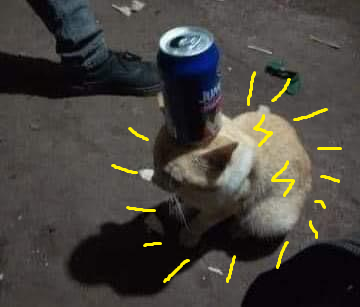
\includegraphics[width=0.5\linewidth]{el.png}
    \caption{Electrogato}
    \label{fig:enter-label}
\end{figure}\\

\begin{thebibliography}{99}

\bibitem{griffiths}
D. J. Griffiths, \textit{Introduction to Electrodynamics}, 3rd ed. Upper Saddle River, NJ, USA: Prentice-Hall, 1999.

\bibitem{jackson}
J. D. Jackson, \textit{Classical Electrodynamics}, 3rd ed. New York, NY, USA: Wiley, 1998.

\bibitem{sadiku}
M. N. O. Sadiku, \textit{Elements of Electromagnetics}, 6th ed. New York, NY, USA: Oxford University Press, 2014.

\bibitem{wangsness}
R. K. Wangsness, \textit{Electromagnetic Fields}, 2nd ed. New York, NY, USA: Wiley, 1986.

\bibitem{zangwill}
A. Zangwill, \textit{Modern Electrodynamics}. Cambridge, UK: Cambridge University Press, 2013.

\bibitem{purcell}
E. M. Purcell and D. J. Morin, \textit{Electricity and Magnetism}, 3rd ed. Cambridge, UK: Cambridge University Press, 2013.

\bibitem{shadowitz}
A. Shadowitz, \textit{The Electromagnetic Field}. Mineola, NY, USA: Dover Publications, 1988.


\end{thebibliography}


\end{document}